\chapter[Configuration Space Approximation using Instance-based Learning]{Configuration Space Approximation \mbox{using} \\ Instance-based Learning} 
\label{chp:IBL}

\section{Introduction}
In motion planning algorithms such as~\cite{Kavraki96, Kuffner00}, the collision detection module is widely used as an oracle to collect information about the free space and approximate its topology. This module is used to classify a given configuration or a local path as either collision-free (i.e., in $\Cfree$) or in-collision (i.e., overlaps with $\Cobs$). Most motion planning algorithms tend to store only the collision-free samples and local paths, and use them to compute a global path from the initial configuration to the goal configuration. Typically, the in-collision configurations or local paths are discarded.

In this chapter, we incrementally construct an approximate $\Cspace$ representation by exploiting all prior or historical information related to collision queries. The approximate $\Cspace$ representation is used to improve the performance of the sample-based planner. Some planners in previous work utilized the in-collision configurations or the samples near the boundary of the configuration obstacles (i.e., $\Ccont$) to bias the sample generation or improve the performance of planners in narrow passages~\cite{Boor:1999:ICRA,Jory:2011:IROS,Rodriguez:2006,Zheng:2005}. However, it can be expensive to perform geometric reasoning based on the outcome of a large number of collision queries in high-dimensional spaces. As a result, most prior planners only use partial or local information about configuration spaces, and can't provide any guarantees in terms of improving the overall performance.
\subsection{Main Results}
We present a novel approach which improves the performance of sample-based planners by having the planners learn from prior instances of collision checking, including all in-collision samples. Our formulation uses the historical information generated using collision queries to compute an approximate representation of $\Cspace$ as a hash table. Given a new probe or collision query in $\Cspace$, we first perform efficient learning on the approximate $\Cspace$ in order to compute a collision probability for this query. This probability is used either as a similarity result or as a prediction of the exact collision query and can improve a planner's efficiency.

The underlying learning process performed on the approximate $\Cspace$ is based on the $\knn$ ($k$-nearest neighbor) queries. All prior configurations used
by the planning algorithm are stored incrementally, along with their collision outcomes, in a hash table. Given a new configuration or a local path, our algorithm computes the nearest neighbors in the hash table. We use locality-sensitive hashing (LSH) algorithms to efficiently perform approximate $\knn$ computations in high-dimensional configuration spaces. Specifically, we present a line-point $\knn$ algorithm that can compute the nearest neighbors of a line.
We derive bounds on the accuracy and time complexity of $\knn$ algorithms and show that the collision probability computed using LSH-based $\knn$ algorithm converges to exact collision detection as the size of dataset increases.

We present improved versions of PRM, lazyPRM and RRT planning methods based on our learning algorithm. Our approach is general and can be combined with any sampling scheme. Furthermore, it is quite efficient for high-dimensional configuration spaces. We have applied these planners to rigid and articulated robots, and have observed up to 100\% speedups based on instance-based learning. Finally, the learned approximate $\Cspace$ can be updated efficiently for moving obstacles and can also be used for motion planning in dynamic environments.

\subsection{Organization}
The rest of this chapter is organized as follows. We survey related work in Section~\ref{sec:3:related}. Section~\ref{sec:3:overview} gives an overview of sample-based planners, LSH-based approximate $\knn$ search and our approach. We present details of the learning process on the $\Cspace$ and analyze its accuracy and complexity in Section~\ref{sec:3:linelsh} and Section~\ref{sec:3:knnreasoning}. We show the integration of the learning algorithm with different motion planning algorithms in Section~\ref{sec:3:planners} and evaluate the performance of the modified planners on various benchmarks in Section~\ref{sec:3:results}.


\section{Related Work}
\label{sec:3:related}

In this section, we give a brief overview of prior work on the use of machine learning techniques in motion planning and on performing efficient collision checking to accelerate sample-based motion planning.

\subsection{Machine Learning in Motion Planning}
Many techniques have been proposed to improve the performance of sample-based motion planning using machine learning. \cite{Marco:2004:WAFR} combine a set of basic PRM motion planners into a powerful `super' planner by assigning different basic planners to different regions in $\Cspace$ based on offline supervised learning. \cite{Burns:2003:ITC,Burns:2005:SQE,Burns-RSS-05} use entropy to measure each sample's utility to improve the coverage of PRM roadmap. \cite{Hsu:2005} adaptively combine multiple sampling strategies to improve the roadmap's connectivity. Some variants of RRT, which use workspace or task-space bias (e.g., \cite{Diankov:2008}), can be extended by changing the bias parameters adaptively.
\cite{Scholz:2010} combine RRT with reinforcement learning. Learning techniques have been used to estimate a zero-measure subspace to bias the sampling in narrow passages, given a sufficient number of collision-free samples~\cite{Dalibard:2011}. Our approach is complimentary to all these techniques.

\subsection{Learning from Experience}
Machine learning can also enable robots to exploit learned knowledge about the underlying geometric structures in tasks and human environments. Many approaches which help robots learn from past experience have been proposed. Most of them can be categorized as planning level methods, usually attempting to reuse the trajectories planned in the past. \cite{Jetchev:2010} construct a database of high-dimensional features which captures information about the proximity of the robot to obstacles; they use such information from the database to predict a good path when facing a new situation.
Other methods construct a database of past motion plans, which can bias the search towards the new planning problem~\cite{Jiang:2007} or to efficiently construct a new plan~\cite{Berenson:2012, Mike:2012}. Plan databases have also been used to adapt policies to new situations or tasks~\cite{Stolle:2006}. The problem of how to select the
most robust set of paths (with respect to unknown obstacle configurations) from the plan database was treated in~\cite{Branicky:2008}.

\subsection{Collision Checking for Motion Planning}
One important feature of sample-based motion planners is the use of exact collision queries to probe the connectivity of $\Cfree$. However, the topology of $\Cfree$ can be rather complex, and may consist of multiple components or small, narrow passages. As a result, it is hard to capture the full connectivity of $\Cfree$ using collision queries. There is extensive work on various techniques to improve the connectivity computation by using different sampling strategies.

Many sampling approaches used for sample-based planners tend to be memoryless, i.e., the sampling technique used to generate the $(n+1)$th sample is independent of the previous $n$ samples. For example,
OBPRM~\cite{Amato:1998:OOP} uses pairs of collision-free and in-collision samples to compute samples near the boundary of $\Cfree$ (or $\Cobs$).
Gaussian sampling~\cite{Boor:1999:ICRA} also generates samples in pairs and a sample is retained when exactly one of the samples in a pair is collision free, therefore resulting in samples that are close to the boundary $\Cobs$. Similar ideas have been used in many variants of RRT, such as retraction-based planners~\cite{Hsu:1998:FNP,Rodriguez:2006,Zhang:2008:ICRA}. \cite{Zheng:2005} identify narrow passages in $\Cspace$ by checking whether a collision-free sample has two in-collision samples nearby. \cite{Kavraki96} use in-collision samples to estimate the visibility of each sample and generate more samples in regions with small visibility. Our approach can be combined with all these techniques to improve the performance of collision checking.

In some recent approaches, adaptive sampling strategies have been proposed that evolve as more information about $\Cspace$ and $\Cfree$ is learned via sampling. In other words, these strategies are not memoryless because the underlying approximate representation of $\Cspace$ changes as more samples are generated. For instance, \cite{Jaillet:2005:IROS} and \cite{Yershova:2005:ICRA} approximate the free space using a set of size-varying balls around nodes in the RRT representation. \cite{Burns-RSS-05} approximate the $\Cspace$ using a set of prior samples, either collision-free or in-collision. These prior samples can predict the collision status for a local path connecting two PRM nodes~\cite{Burns:2005:ICRA}. Recently, \cite{Knepper:2012:IJRR} extend the adaptive sampling approach in~\cite{Burns-RSS-05} to non-holonomic motion planning by defining the utility of local paths. \cite{Jory:2011:IROS} construct roadmaps in both $\Cfree$ and $\Cobs$, which are used to generate more samples in narrow passages.


\subsection{$k$-Nearest Neighbor Search}
The problem of finding the $k$-nearest neighbor within a database of high-dimensional points is well-studied in various areas, including databases, computer vision, and machine learning. Samet's book~\cite{Samet:2005:FMM} provides a good survey of various techniques used to perform the $\knn$ search. In order to handle large and high-dimensional spaces, most practical algorithms are based on approximate $\knn$ queries~\cite{Chakrabarti:FOCS}. In these formulations, the algorithm is allowed to return a point whose distance from the query point is at most $1+\epsilon$ times the distance from the query to its $k$-nearest points; $\epsilon > 1$ is called the \emph{approximation factor}. LSH-based $\knn$ has already been used in motion planning, e.g., a parallel version of LSH-based $\knn$ was used in a parallel PRM framework~\cite{Pan:IROS:2010}. Please refer to Chapter~\ref{chp:GLSH} for a more detailed background and discussion about LSH-based $\knn$.



\section{Overview}
\label{sec:3:overview}
In this section, we give an overview of the sample-based planner and provide a brief background on the learning algorithm we used to improve the motion planner.


\subsection{Notations and Symbols}
In this chapter, we denote each point configuration with $\Cspace$ as $\mathbf x$. We use $\mathcal D$ to denote a set of $N$ configuration points $\mathcal D = \{\mathbf x_1, \mathbf x_2, ... \mathbf x_N\}$ along with their exact collision statuses, which is an approximation of the exact $\Cspace$.

A \emph{local path} in $\Cspace$ is a continuous curve that connects two configurations.
It is difficult to compute $\Cobs$ or $\Cfree$ explicitly; therefore, sample-based planners use collision checking between the robot and obstacles to probe the $\Cspace$ implicitly. These planners perform two kinds of queries: the \emph{point query} and the \emph{local path query}. We use the symbol $Q$ to denote either of these queries. When it is necessary to distinguish point and line queries, we use $\mathbf p$ for a point query and $l$ for a line query.

We denote $\dist(\cdot, \cdot)$ to be a distance metric over the items in $\Cspace$, i.e., the distance between two points $\mathbf x$ and $\mathbf x'$ is $\dist(\mathbf x, \mathbf x')$. We use $B(\mathbf x, r)$ to denote the set of points from $\Cspace$ whose distances to $\mathbf x$ is smaller than $r$, where the distance is computed according to metric $\dist(\cdot, \cdot)$. In other words, $B(\mathbf x, r) = \{\mathbf x' \in \Cspace: \dist(\mathbf x, \mathbf x') \leq r\}$. We also use the symbol $e$ to denote the base of the natural logarithm.

We use operator $y(\cdot)$ to denote the exact collision status ($0$ for collision-free and $1$ for in-collision). In particular, $y(\mathbf x)$ is the collision status of a configuration sample $\mathbf x$, $y(\mathbf p)$ is the collision status of a point query, and $y(l)$ is the collision status of a line. We usually abbreviate $y(\mathbf x)$ or $y(\mathbf p)$ by $y$. The estimated collision status of a query is computed by a binary-class classifier $c(\cdot)$.

We denote $\vectorize(\cdot)$ as the vectorization of a given matrix. In particular, $\vectorize(\mathbf A)$, the vectorization of an $m\times n$ matrix $\mathbf A$, is the $m n \times 1$ column vector which is obtained by stacking the columns of the matrix $\mathbf A$ on top of one another:
\begin{equation}
  \vectorize(\mathbf A) = [a_{1,1}, ..., a_{m,1}, a_{1,2}, ..., a_{m,2}, ..., a_{1,n}, ..., a_{m,n}]^T, \notag
\end{equation}
where $a_{i,j}$ represents the $(i,j)$-th element of matrix $\mathbf A$.


\subsection{Enhanced Motion Planner with Instance-based Learning}
The goal of a motion planner is to compute a collision-free continuous path between the initial and goal configurations in $\Cspace$. The resulting path should lie completely in $\Cfree$ and should not intersect with $\Cobs$. As shown in Figure~\ref{fig:3:oracle}(a), sample-based planners learn about the connectivity of $\Cspace$ implicitly based on collision queries. The query results can also bias the sampling scheme of the planner via different heuristics (e.g., retraction rules).

\emph{Instance-based learning} is a well-known family of algorithms in machine learning. These algorithms learn properties of new problem instances by comparing them with the instances observed earlier that have been stored in memory~\cite{Russell:2003}. In our case, we store all the results of prior collision queries, including collision-free as well as in-collision queries. Our goal is to sufficiently exploit this prior information to accelerate the planner computation. The problem instance in our context is the collision query being performed on a given configuration or a local path in $\Cspace$. In particular, performing exact collision queries for local planning can be expensive. Collision checking for a discrete configuration is relatively cheap, but still can be time-consuming if the environment or the robot's geometric representation has a high complexity. We utilize the earlier instances or the stored information by performing $\knn$ queries and geometric reasoning on query results.

Our new approach exploits prior information for motion planning, as shown in Figure~\ref{fig:3:oracle}(b). When the collision checking routine finishes probing the $\Cspace$ for a given query, it stores all the obtained information in a dataset $\mathcal D$ corresponding to historical collision query results. If the query is a point within $\Cspace$, the stored information is its binary collision status. If the query is a local path, the stored information includes the collision status of different configuration points along the path. The resulting dataset of historical collision results constitutes the complete set of information we have about $\Cspace$, all learned from collision checking routines. Therefore, we use it as an approximate description of the underlying $\Cspace$: the in-collision samples are an approximation of $\Cobs$, while the collision-free samples are used to encode $\Cfree$. These samples are used by instance-based learning algorithms to estimate the collision status of new queries.

Given a new query $Q$, either a point or a local path, we first perform $\knn$ search on the dataset $\mathcal D$ to find its neighbor set $S$, which provides information about local $\Cspace$ around the query $Q$. If $S$ contains sufficient information to infer the collision status of the query, we compute a collision probability for the new query based on $S$; otherwise, we perform exact collision checking for this query and the query result is added into $\mathcal D$. The calculated collision probability provides prior information about the collision status of a given query, and is used in different ways. First, it can be used as a culling filter to avoid the exact (and expensive) collision checking for queries that correspond to the configurations or local paths located in regions that are well sampled and approximated in the database. Secondly, it can decide an efficient order in which to perform exact collision checking for a set of queries. For example, many planners like RRT need to select the local path that can best improve the local exploration in $\Cfree$, i.e., a local path that is both long and collision-free. The collision probability computation can compute an efficient sorting strategy, which thereby reduces the number of exact collision tests.

The notion of having sufficient information about $S$ (in Algorithm~\ref{algo:3:collisionquery}) is related to how much confidence we have in our inferences drawn from $S$. If the confidence is too small, the algorithm rejects the results of approximate collision queries and performs exact collision queries instead.
We consider two types of rejection cases: \emph{ambiguity rejection} and \emph{distance rejection}~\cite{Dubuisson:1993:PR}. Ambiguity rejection happens when the collision probability of a given query is nearly 0.5. Distance rejection happens when the query configuration is far (in terms of geometric distance) from all prior instances stored in the database.

A description of our learning-based collision framework is given in Algorithm~\ref{algo:3:collisionquery}, which is used as an inexpensive routine to perform probabilistic or approximate collision detection. More details about this routine and its applications are given in Section~\ref{sec:3:linelsh} and Section~\ref{sec:3:knnreasoning}.




\begin{algorithm}[htb]
    \caption{\texttt{learning-based-collision-query}($\mathcal D, Q$)}
    \label{algo:3:collisionquery}
    \begin{algorithmic}[1]
	\IF{$Q$ \emph{is point query}}
	   	   \STATE $S \leftarrow $ \texttt{point-point-$\knn$}($Q$)
           \IF{$S$ \emph{provides sufficient information for reasoning}}
				\STATE \texttt{approximate-collision-query}($S, Q$)
		   \ELSE
				\STATE \texttt{exact-collision-query}($\mathcal D, Q$)
           \ENDIF
   \ENDIF
   \IF{$Q$ \emph{is line query}}
              \STATE  $S \leftarrow $ \texttt{line-point-$\knn$}($Q$)
              \IF{$S$ \emph{provides sufficient information for reasoning}}
				   \STATE \texttt{approximate-continuous-collision-query}($S, Q$)
			  \ELSE
                    \STATE \texttt{exact-continuous-collision-query}($\mathcal D, Q$)
              \ENDIF
\ENDIF
	    \end{algorithmic}
\end{algorithm}


\begin{figure}[htb]
  \centering
  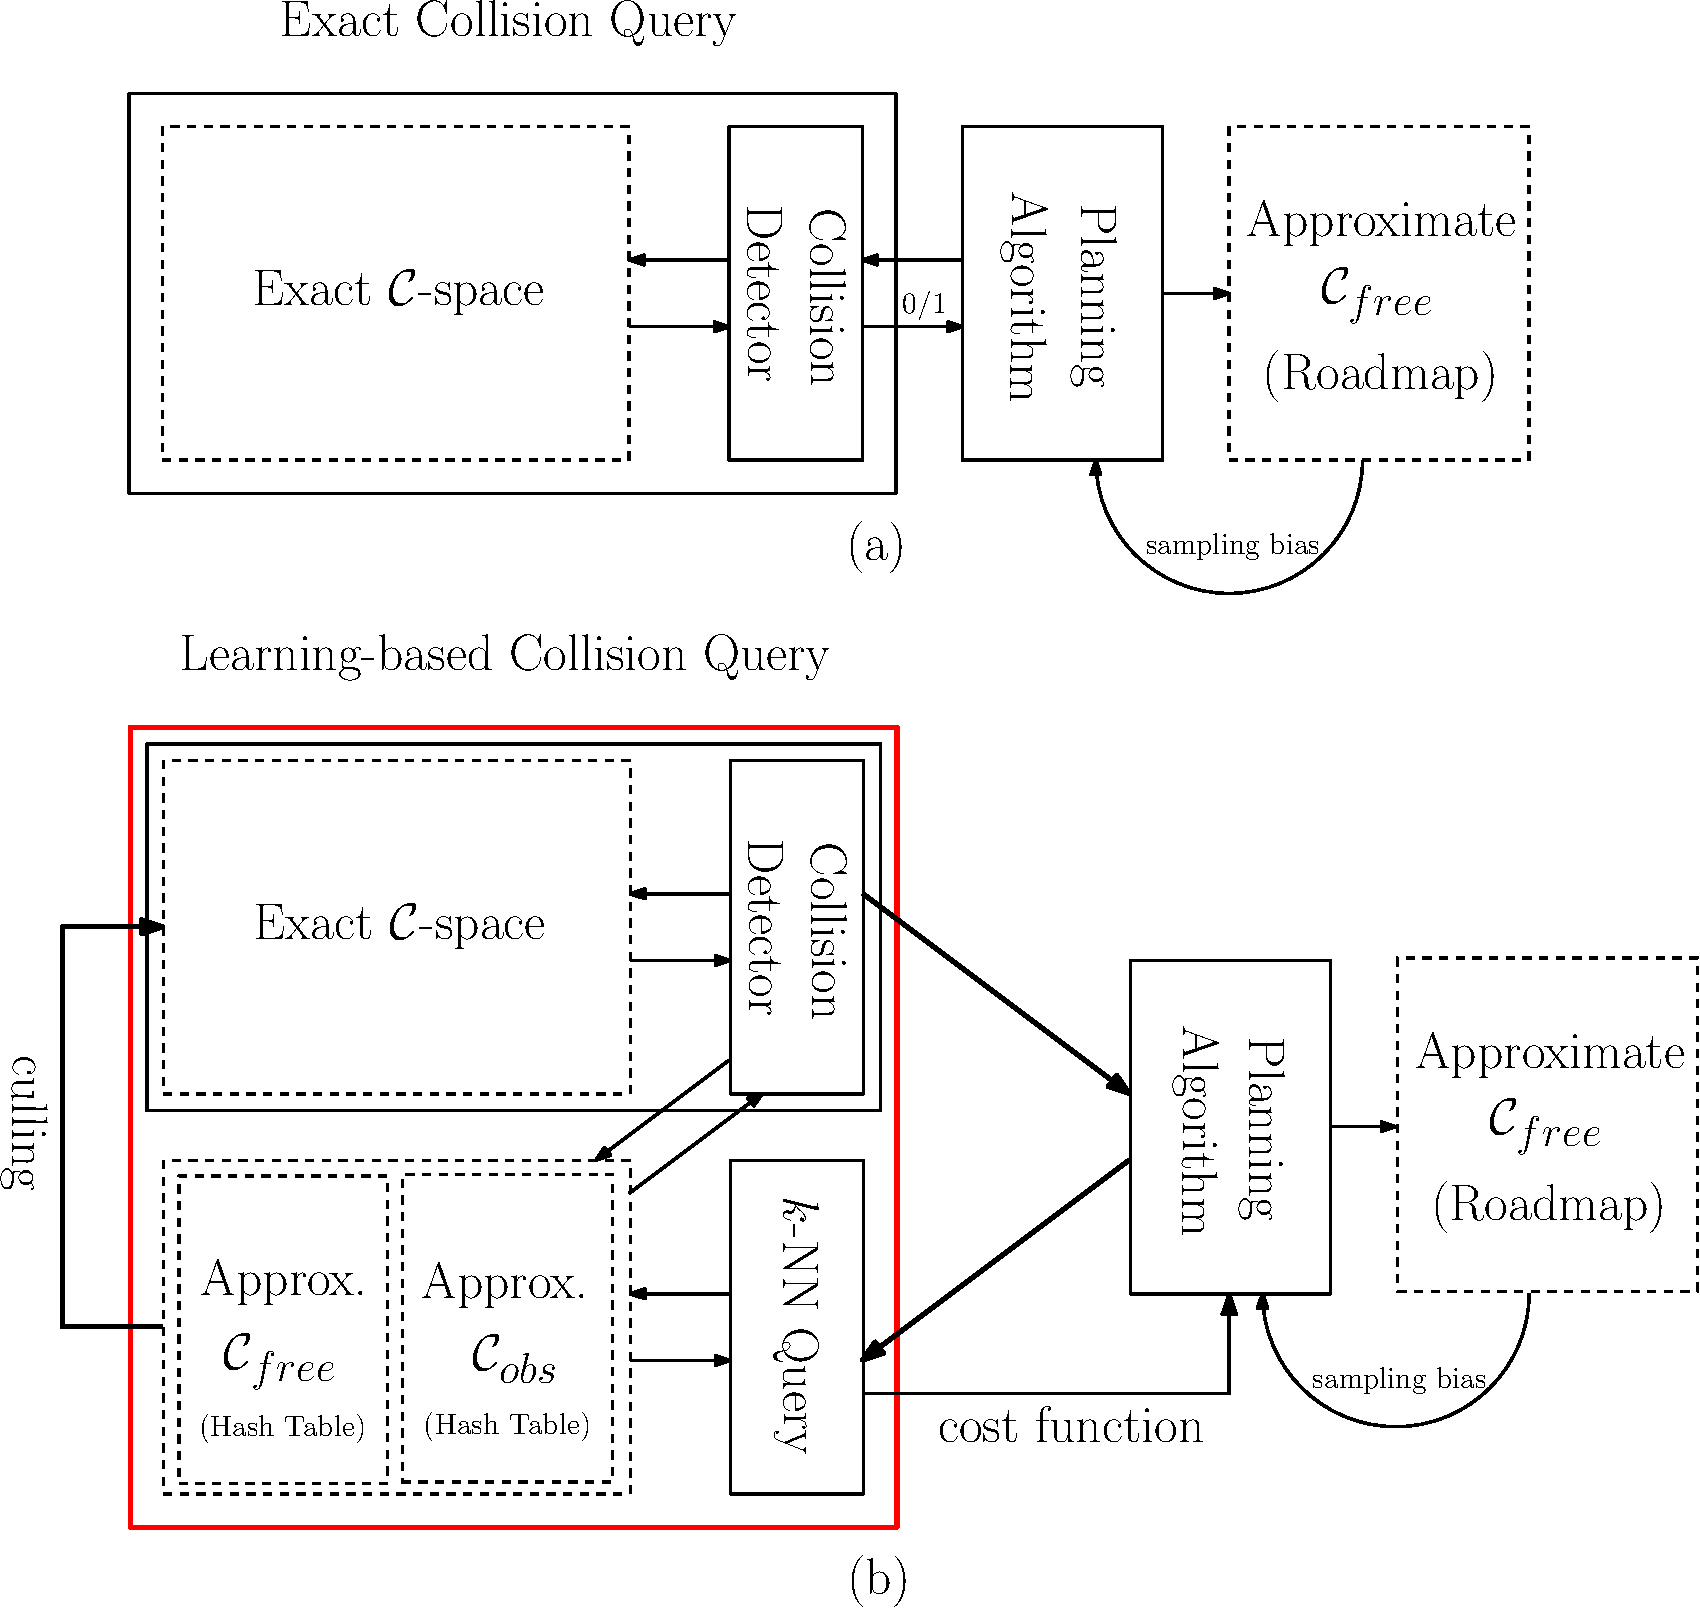
\includegraphics[width=\linewidth]{figs/3/oracle.pdf}
  \caption[Comparison between prior sample-based planners and planners enhanced by instance-based learning]{Use of collision detection in sample-based planners: exact collision checking only (a) and our approach with exact and approximate collision checking (b). (a) The collision detection routine is the oracle used by the planner to gather information about $\Cfree$ and $\Cobs$. The planner performs binary collision queries, either on point configurations or $1$-dimensional local paths, and estimates the connectivity of $\Cfree$ (shown as Approximate $\Cfree$). Moreover, some planners utilize the in-collision results to bias sample generation by using different heuristics. (b) Our method also performs collision queries. However, we store all in-collision results (as Approximate $\Cobs$) and collision-free results (as Approximate $\Cfree$). Before performing an exact collision query, our algorithm performs a $\knn$ query on the given configuration or local path to compute a collision probability for each query. The collision probability can be used as a cost function to compute an efficient strategy for performing exact collision queries during motion planning. We use novel LSH-based algorithms to perform $\knn$ queries efficiently and to speed up the overall planner.}
  \label{fig:3:oracle}
\end{figure}


\subsection{LSH-based Approximate $\knn$ Query}
\label{sec:3:overview:lsh}
A key issue for our learning framework is its computational efficiency. As we generate hypotheses directly from training instances, the complexity of this computation can grow with the size of historical data. If we use exact $\knn$ computation as the underlying learning method, its complexity can be a linear function of the size of the dataset, especially for high-dimensional spaces. To improve the efficiency of the instance-based learning, we use approximate $\knn$ algorithms.

Given a dataset $\mathcal D = \{\mathbf x_1, \mathbf x_2, ... \mathbf x_N\}$ of $N$ points in $\mathcal R^d$, we consider two types of retrieval queries. One retrieves the points from $\mathcal D$ closest to a given point query: this is the well-known $\knn$ query, which we call the \emph{point-point $\knn$} query. The second query tries to find the points from $\mathcal D$ that are closest to a given line in $\mathcal R^d$ whose direction is $\mathbf v$ and which passes through a point $\mathbf a$, where $\mathbf v, \mathbf a \in \mathcal R^d$. We call this second query the \emph{line-point $\knn$} query. The two types of $\knn$ queries are illustrated in Figure~\ref{fig:3:KNN}.


In order to develop an efficient instance-based learning framework, we use locality-sensitive hashing (LSH) as an approximate method for $\knn$ queries, which is mainly designed for point-point queries~\cite{Andoni:2008:NHA}. However, it can be extended to line queries~\cite{Andoni:2009:ALN} and hyper-plane queries~\cite{Jain:nips:2010}. \cite{Basri:2011} further extend it to perform point/subspace queries.

LSH requires randomized hash functions which can guarantee that the probability of two points being mapped into the same hash bucket is inversely proportional to the distance between them. In these cases, the distance metric is defined based on the specific task or application. Since two similar points are likely to fall into nearby hash buckets, we only need to perform a local search within the bucket that contains the given query.


\begin{definition}
\label{def:3:lsh}
  \cite{Andoni:2008:NHA} Let $h_{\mathcal H}$ denote a random choice of hash functions from the function family $\mathcal H$, and let $B(\mathbf x, r)$ be a radius-$r$ ball centered at $\mathbf x$.  $\mathcal H$ is called $(r, r(1+\epsilon), p_1, p_2)$-sensitive for $\dist(\cdot, \cdot)$ when for any $\mathbf x$, $\mathbf x' \in \mathcal D$,
  \begin{itemize}
  \item if $\mathbf x' \in B(\mathbf x, r)$, then $\mathbb P[h_{\mathcal H}(\mathbf x) = h_{\mathcal H}(\mathbf x')] \geq p_1$,
  \item if $\mathbf x' \notin B(\mathbf x, r(1+\epsilon))$, then $\mathbb P[h_{\mathcal H}(\mathbf x) = h_{\mathcal H}(\mathbf x')] \leq p_2$.
  \end{itemize}
\end{definition}
For a family of functions to be useful, we require $p_1 > p_2$.

A higher dimensional hash function $g$ can be constructed by concatenating several hash functions randomly selected from the function family $\mathcal H$: $g(\mathbf x) = [h_{\mathcal H}^{1}(\mathbf x), h_{\mathcal H}^{2}(\mathbf x), ..., h_{\mathcal H}^{M}(\mathbf x)]$, where $M$ is the dimension of $g$.
Given the hash function $g$, the hashing collision probability for two close points is at least $(p_1)^M$, while for dissimilar points it is at most $(p_2)^M$. Each item in the dataset $\mathcal D$ is mapped to a series of $L$ hash tables indexed using independently constructed functions $g_1, ..., g_L$, where each $g_i$ is a dimension-$M$ function. Next, given a point query $\mathbf p$, an exhaustive search is carried out only on the items in the union of the $L$ buckets. These candidates constitute the $(r,\epsilon)$-nearest neighbor for $\mathbf p$, meaning that if $\mathbf p$ has a neighbor within radius $r$, then with high probability some item within radius $r(1+\epsilon)$ would be found. When $\dist(\cdot, \cdot)$ corresponds to the $l_2$ metric, we have following result about point-point $\knn$ query:
\begin{theorem}
  \label{thm:3:pplsh}
  (Point-point $\knn$ query) \cite{Datar:2004:LHS} Let $\mathcal H$ be a family of $(r, r(1+\epsilon), p_1, p_2)$-sensitive hash functions, with $p_1 > p_2$. Given a dataset of size $N$, we set $M = \log_{1/p_2} N$ and $L = N^{\rho}$, where $\rho = \frac{\log p_1}{\log p_2}$. Using $L$-hash tables over dimension $M$, given a point query $\mathbf p$, with probability at least $\frac{1}{2} - \frac{1}{e}$, the LSH algorithm solves the $(r, \epsilon)$-neighbor problem. In other words, if there exists a point $\mathbf x$ that $\mathbf x \in B(\mathbf p, r(1+\epsilon))$, then the algorithm will return the point with probability $\geq \frac{1}{2} - \frac{1}{e}$. The retrieval time is bounded by $\mathcal O(N^{\rho})$.
\end{theorem}

If we choose $\mathcal H$ to be the hamming hash or $p$-stable hash:
\begin{equation}
  \begin{aligned}
    \label{eq:3:hashfunc}
    \{h^{\mathbf u} : h^{\mathbf u}(\mathbf x) = \sign(\mathbf u^T \mathbf x)\} \text{\ or\ } \{h^{\mathbf a, b} : h^{\mathbf a, b}(\mathbf x) = \lfloor \frac{\mathbf a^T \mathbf x + b}{W}\rfloor\},
  \end{aligned}
\end{equation}
where $\mathbf u$ and $\mathbf a \sim \mathcal N(\mathbf 0, \mathbf I)$, $b \sim \mathcal U[0, W]$ and $W$ is a fixed constant, we have $\rho \leq \frac{1}{1+\epsilon}$ and the algorithm has sub-linear complexity, i.e., the results can be retrieved in time $\mathcal O(N^{\frac{1}{1+\epsilon}})$.


We build on these prior results for point-point $\knn$ queries; we present a new LSH-based algorithm for line-point $\knn$ queries. The LSH parameters (e.g., $\mathbf u$, $W$, $\mathbf a$ and $b$ in Equation~\ref{eq:3:hashfunc}) are chosen randomly a-priori. When the collision result for a new configuration query is computed, we calculate the hash code for that query and add it to the hash tables. This operation is is performed once for each item stored in the database.

Later in Section~\ref{sec:3:linelsh}, we discuss issues in designing appropriate hash functions for line-point $\knn$ queries, and we derive LSH bounds for line-point $\knn$. We also address many issues in extending our formulation to non-Euclidean metrics (e.g., in handling articulated models) and reducing the dimension of embedded space.

\begin{figure}[htb]
  \centering
  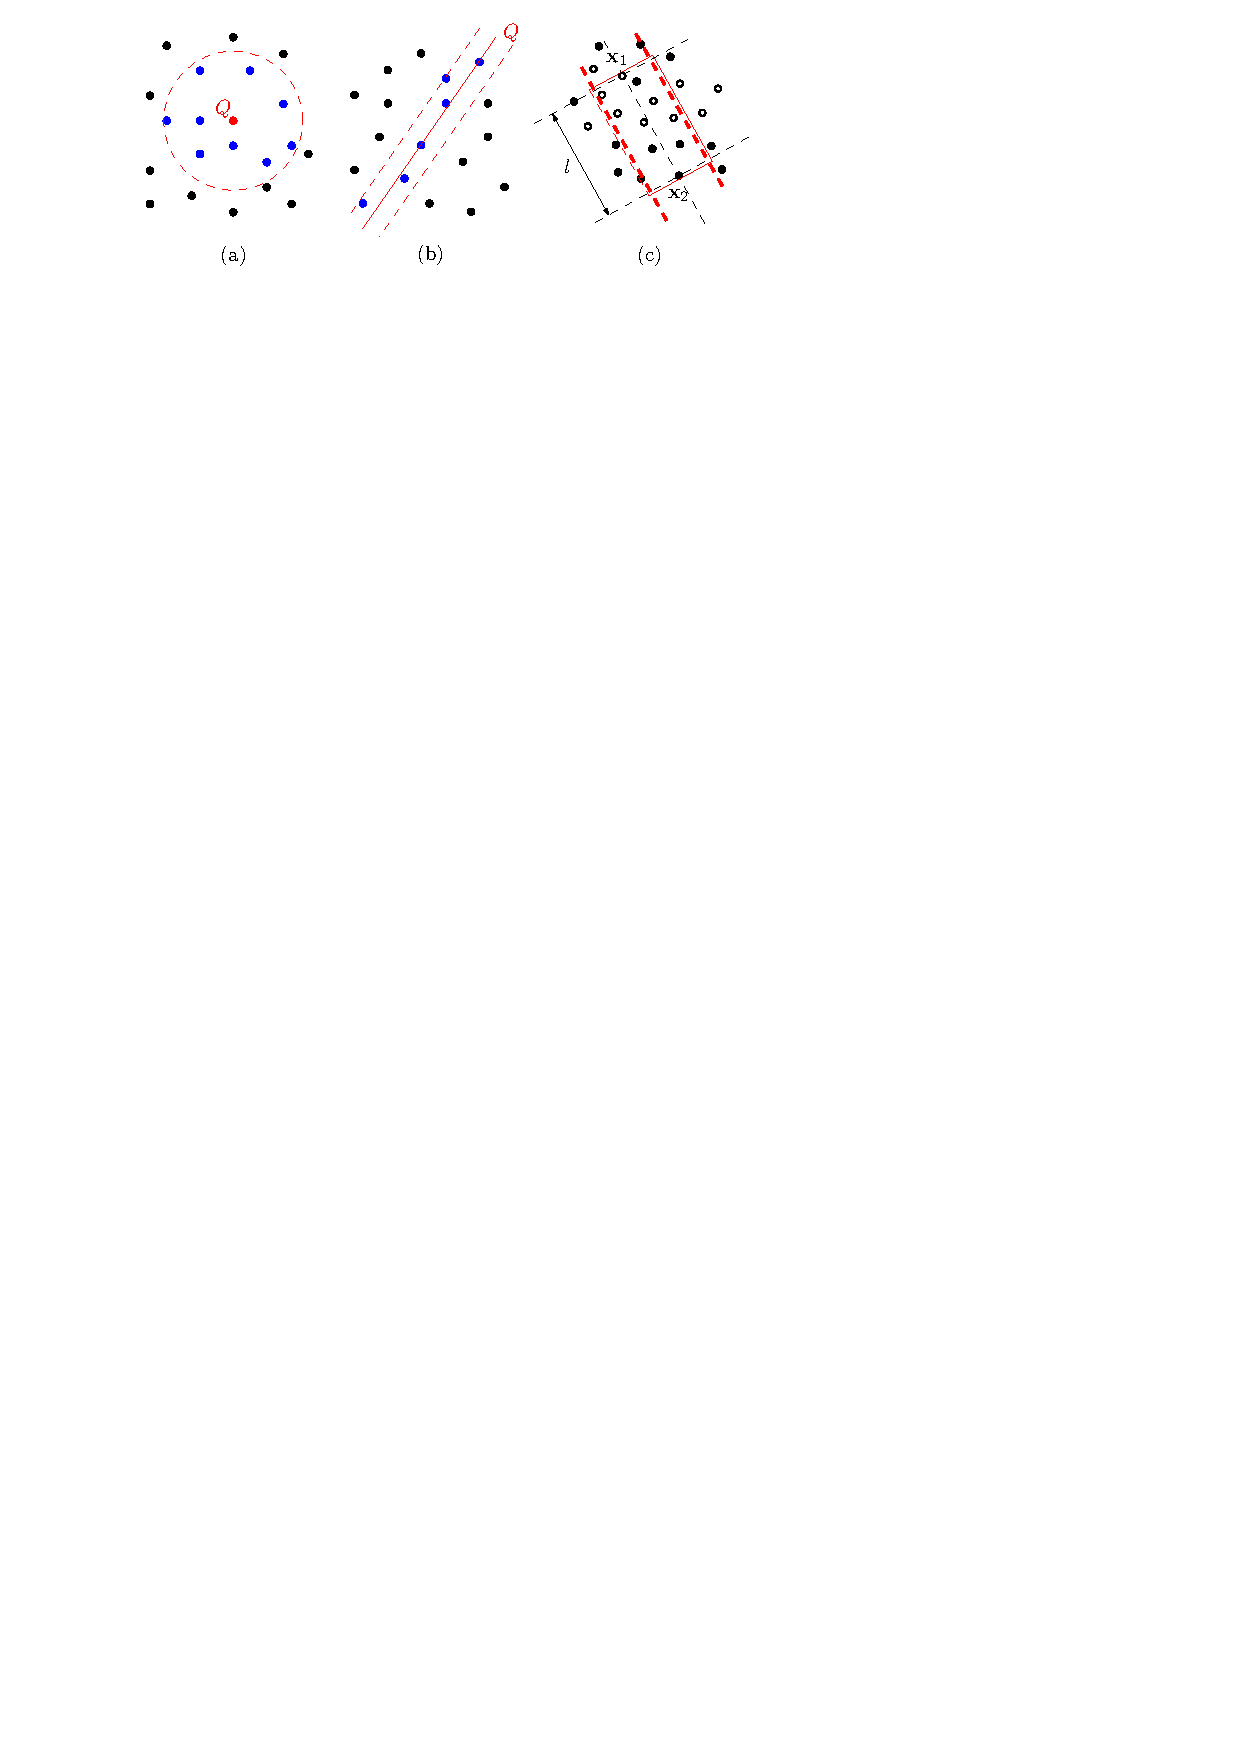
\includegraphics[width=\linewidth]{figs/3/KNN.pdf}
  \caption[Two types of $\knn$ queries used in instance-based learning]{Two types of $\knn$ queries used in our method: (a) point-point $\knn$; (b) line-point $\knn$. $Q$ is the query item, and the results of different queries are shown as blue points in each figure. We present novel LSH-based algorithms for fast computation of these queries. (c) The line-point $\knn$ query is used to compute prior instances that can influence the collision status of a local path which connects $\mathbf x_1$ and $\mathbf x_2$ in $\Cspace$. The query line is the line segment between $\mathbf x_1$ and $\mathbf x_2$. The white points are prior collision-free samples in the dataset, and the black points are prior in-collision samples.}
  \label{fig:3:KNN}
\end{figure}





\section{LSH-based Line-Point $\knn$ Query}
\label{sec:3:linelsh}
One of the contributions of this chapter is to extend the LSH formulation to the line-point $\knn$ query, which is used to efficiently estimate the collision status of a local path. In comparison with previous methods for such computations~\cite{Andoni:2009:ALN,Basri:2011}, our line-point $\knn$ results in a more compact representation; we also derive LSH bounds similar to the point-point $\knn$, as shown in Theorem~\ref{thm:3:pplsh}. Moreover, we address several issues that arise when using our algorithm for sample-based motion planning, such as handling non-Euclidean metrics and reducing the dimension of the embedded space.

The simplest algorithm for line-point $\knn$ query is based on sampling the line into a sequence of uniformly sampled points at a fixed resolution, and using point-point $\knn$ algorithms on each of those sampled points. One major drawback of using such an approach is its efficiency, as we land up performing a high number of point-point $\knn$ queries for a given line or local path. Furthermore, the samples in the database are typically not distributed in a uniform manner. As a result, it is hard to compute the appropriate sampling resolution for the line.

The main issue in terms of using LSH to perform line-point $\knn$ query is to embed the line query and the point dataset into a higher-dimensional space, and then to perform point-point $\knn$ queries in that embedded space. First, we present a technique to perform line-point embedding. Next, we design hash functions for the embedding and prove that these hash functions satisfy the locality-sensitive property for the original data (i.e., $\mathcal D$). Finally, we derive the error bound and time bound for the approximate line-point $\knn$ query, which is similar to that given in Theorem~\ref{thm:3:pplsh}.

\subsection{Line-point Distance}
A line $l$ in $\mathcal R^d$ is described as $l = \{\mathbf a + s \cdot \mathbf v\}$, where $\mathbf a$ is a point in $\mathcal R^d$ and $\mathbf v$ is a unit vector in $\mathbf R^d$.
The Euclidean distance of a point $\mathbf x \in \mathcal R^d$ to the line $l$ is given as:
\begin{equation}
\label{eq:3:basicdist}
  \dist^2(\mathbf x, l) = (\mathbf x - \mathbf a) \cdot (\mathbf x - \mathbf a) - ((\mathbf x - \mathbf a) \cdot \mathbf v)^2.
\end{equation}
Given a database $\mathcal D = \{\mathbf x_1, ..., \mathbf x_N\}$ of $N$ points in $\mathcal R^d$, the goal of line-point $\knn$ query is to retrieve the points from $\mathcal D$ that are closest to $l$. We do not directly use Equation~\ref{eq:3:basicdist} for line-point $\knn$ query, because in that form the database item (i.e., the point) and the query item (i.e., the line) are not well separated. To accelerate the line-point $\knn$ using LSH-based techniques, we transform the distance metric to a form which is more suitable for efficient $\knn$ query.

\subsection{Line-point Embedding: Non-affine Case}
\label{subsubsec:3:embed}
We first assume the non-affine line query, i.e., $l$, passes through the origin (i.e., $\mathbf a = \mathbf 0$). In this case, $\dist(\mathbf x, l) = \mathbf x \cdot \mathbf x - (\mathbf x \cdot \mathbf v)^2$. This distance can be re-formalized as the inner product of two $(d+1)^2$-dimensional vectors:
\begin{align}
  \label{eq:3:dist}
  &\quad{} \dist^2(\mathbf x, l) \notag \\
  &= \mathbf x \cdot \mathbf x - (\mathbf x \cdot \mathbf v)^2 \notag \\
  &= \vectorize(\begin{pmatrix} \mathbf I & \mathbf 0 \end{pmatrix}^T (\mathbf I - \mathbf v \mathbf v^T) \begin{pmatrix} \mathbf I & \mathbf 0 \end{pmatrix}) \cdot \vectorize(\begin{pmatrix} \mathbf x \\ t \end{pmatrix} \begin{pmatrix} \mathbf x \\ t \end{pmatrix}^T) \\
  &= V^P(\mathbf v) \cdot V^L(\mathbf x), \notag
\end{align}
where $\mathbf I$ is $d\times d$ identity matrix, $\trace(\cdot)$ is the trace of a given square matrix and $t$ can be any real value; $\vectorize(\cdot)$ is the vectorization operation. $V^P(\cdot)$ is an embedding which yields a $(d+1)^2$-dimensional vector from $d$-dimensional point vector $\mathbf x$: $V^P(\mathbf x) =
\vectorize(\begin{pmatrix} \mathbf x \\ t \end{pmatrix} \begin{pmatrix} \mathbf x \\ t \end{pmatrix}^T)$; $V^L(\cdot)$ is an embedding which yields a $(d+1)^2$-dimensional vector from a line $l = \{s \mathbf v\}$ in $d$-dimensional space: $V^L(\mathbf v) = \vectorize(\begin{pmatrix} \mathbf I - \mathbf z \mathbf v^T & \mathbf 0 \\ \mathbf 0^T & 0 \end{pmatrix})$.

Moreover, we notice that the Euclidean distance between the embedding $V^P(\mathbf x)$ and $-V^L(\mathbf v)$ is given by
\begin{equation}
  \begin{aligned}
    \label{eq:3:embed}
    &\quad{} \|V^P(\mathbf x) - (- V^L(\mathbf v)) \|^2 \\
    &= d - 1 + \|V^P(\mathbf x)\|^2 + 2(V^P(\mathbf x) \cdot V^L(\mathbf v)) \\
    &= d - 1 + (\|\mathbf x\|^2 + t^2)^2 + 2\dist^2(\mathbf x, l).
  \end{aligned}
\end{equation}
In Equation~\ref{eq:3:embed}, if the term $d - 1 + (\|\mathbf x\|^2 + t^2)^2$ is constant, then the point-to-line distance $\dist(\mathbf x, l)$ can be formalized as the distance between two points $V^P(\mathbf x)$ and $-V^L(\mathbf v)$ in the higher-dimensional embedded space. This is possible because $t$ is a free variable that can be chosen arbitrarily. In particular, we choose $t$ as a function of $\mathbf x$: $t(\mathbf x) = \sqrt{c - \mathbf \|x\|^2}$, where $c > \max_{\mathbf x \in \mathcal D}\|\mathbf x\|^2$ is a constant real value related to the entire database $\mathcal D$ but independent from each single item in the database. Then Equation~\ref{eq:3:embed} reduces to $\|V^P(\mathbf x) - (- V^L(\mathbf v)) \|^2 = 2 \dist^2(\mathbf x, l) + \text{constant}$.

Until now, we have successfully separated the database item (i.e., $\mathbf x$) from the query item (i.e., $l$). Next, we can pre-compute the locality-sensitive hash values for all the database items (see Section~\ref{sec:3:linelsh:lshhash}), which are used for efficient line-point $\knn$ computation of any given line queries. Moreover, this reduction implies that we can reduce the line-point $\knn$ query in a $d$-dimensional database $\mathcal D$ to a point $\knn$ query in a $(d+1)^2$-dimensional embedded database $V^P(\mathcal D) = \{V^P(\mathbf x_1), ..., V^P(\mathbf x_N) \}$, where the query item corresponds to $-V^L(\mathbf v)$.

\subsection{Line-point Embedding: Affine Case}
Now we consider the case of any arbitrary affine line, i.e., $\mathbf a \neq \mathbf 0$. Similarly to Equation~\ref{eq:3:dist}, we obtain
\begin{align}
  \label{eq:3:dist2}
   & \dist^2(\mathbf x, l) \notag \\
  =& \ (\mathbf x - \mathbf a) \cdot (\mathbf x - \mathbf a) - ((\mathbf x - \mathbf a) \cdot \mathbf v)^2 \notag  \\
  =& \ \trace(\begin{pmatrix} \mathbf x \\ 1 \\ t \end{pmatrix} ^T \underbrace{\begin{pmatrix} \mathbf I & - \mathbf a & \mathbf 0 \end{pmatrix}^T (\mathbf I - \mathbf v \mathbf v^T) \begin{pmatrix} \mathbf I & -\mathbf a & \mathbf 0 \end{pmatrix}}_{\mathbf B} \begin{pmatrix} \mathbf x \\ 1 \\ t \end{pmatrix}) \notag \\
  =& \ \vectorize(\begin{pmatrix} \mathbf x \\ 1 \\ t \end{pmatrix} \begin{pmatrix} \mathbf x \\ 1 \\ t \end{pmatrix}^T) \cdot \vectorize(\mathbf B) \\
  =& \ \hat{V}^P(\mathbf x) \cdot \hat{V}^L(\mathbf v, \mathbf a), \notag
\end{align}
where $\hat{V}^P(\mathbf x)$ and $\hat{V}^L(\mathbf v, \mathbf a)$ are $(d+2)^2$-dimensional embeddings for a point and line in $\mathcal R^d$, respectively. Similarly to Equation~\ref{eq:3:embed}, if we choose $t(\mathbf x) = \sqrt{c - \mathbf x^2 - 1}$, where $c > \max_{\mathbf x \in \mathcal D} \|\mathbf x\|^2 + 1$ is a constant related to the entire database $\mathcal D$ (i.e., set $\|\hat{V}^P(\mathbf x)\|^2 = c^2$), then $\dist^2(\mathbf x, l)$ also linearly depends on the squared Euclidean distance between the embedded database and the query item: $\|\hat{V}^P(\mathbf x) - \hat{V}^L(\mathbf v, \mathbf a)\|^2 = c^2 + d - 2 + (\dist^2(\mathbf 0, l) + 1)^2 + 2 \dist^2(\mathbf x, l)$. As a result, we can perform an affine line-point $\knn$ query based on a point $\knn$ query in a $(d+2)^2$-dimensional database $\hat{V}^P(\mathcal D) = \{\hat{V}^P(\mathbf x_1), ..., \hat{V}^P(\mathbf x_N) \}$, and the corresponding query item is $-\hat{V}^L(\mathbf v, \mathbf a)$.

%The dimension of the embedded space (i.e., $(d+1)^2$ or $(d+2)^2$) is much higher than the original space (i.e., $d$), and will slow down the LSH computation. We present two techniques to reduce the dimension of the embedded space.
%
%First, notice that the matrices used within $\vectorize(\cdot)$ are symmetric matrices. For a $d \times d$ matrix $\mathbf A$, we can define a $d(d+1)/2$-dimensional embedding $\widehat{\vectorize}(\mathbf A)$ as follows
%\begin{equation}
%  \widehat{\vectorize}(\mathbf A) = [\frac{a_{1,1}}{\sqrt{2}}, a_{1,2}, ..., a_{1,d}, \frac{a_{2,2}}{\sqrt{2}}, a_{2,3}, ..., \frac{a_{d,d}}{\sqrt{2}}]^T.
%\end{equation}
%It is easy to see that $\|\vectorize(\mathbf A) - \vectorize(\mathbf B)\|^2 = 2 \|\widehat{\vectorize}(\mathbf A) - \widehat{\vectorize}(\mathbf B)\|^2$ and hence this dimension-reduction will not influence the accuracy of the line-point $\knn$ algorithm introduced above.
%
%Secondly, we can use the Johnson-Lindenstrauss lemma~\cite{Li:2006:VSR} to reduce the dimension of the embedded data by randomly projecting the high-dimensional embedded data items onto a lower dimensional space. Compared to the first approach, this method can generate an embedding with lower dimensions, but according to our experimental results, it may reduce the accuracy of the line-point $\knn$ algorithms.


\subsection{Locality-Sensitive Hash Functions for Line-Point Query}
\label{sec:3:linelsh:lshhash}
We design the hash function $\hat{h}$ for the line-point query as follows:
\begin{equation}
  \label{eq:3:lphash}
  \begin{cases}
    \hat{h}(\mathbf x) = h(\hat{V}^P(\mathbf x)), & \mathbf x \text{ is a database point} \\
    \hat{h}(l) = h(-\hat{V}^L(\mathbf v, \mathbf a)), & l \text{ is a line }\{\mathbf a + s \cdot \mathbf v\},
  \end{cases}
\end{equation}
where $h$ is a locality-sensitive hash function as defined in Section~\ref{sec:3:overview:lsh}. The new hash functions are locality-sensitive for line-point query, as shown by the following two theorems:
\begin{theorem}
  \label{thm:3:hamminghash}
  The hash function family $\hat{h}$ is $(r, r(1+\epsilon), p_1, p_2)$-sensitive if $h$ is the hamming hash, (i.e., $h = h^{\mathbf u}$), where $p_1 = \frac{1}{\pi} \cos^{-1}(\frac{r^2}{C})$, $p_2 = \frac{1}{\pi} \cos^{-1}(\frac{r^2(1+\epsilon)^2}{C})$ and $C$ is a value independent of database point, but is related to the query. Moreover, $\frac{1}{(1+\epsilon)^2} \leq \rho = \frac{\log p_1}{\log p_2} \leq 1$.
\end{theorem}

\begin{theorem}
  \label{thm:3:pstablehash}
  The hash function family $\hat{h}$ is $(r, r(1+\epsilon), p_1, p_2)$-sensitive if $h$ is the $p$-stable hash, (i.e., $h = h^{\mathbf a, b}$), where $p_1 = f(\frac{W}{\sqrt{2r^2+C}})$ and $p_2 = f(\frac{W}{\sqrt{2r^2(1+\epsilon)^2+C}})$ and $C$ is a value independent of database point, but is related to the query. The function $f$ is defined as $f(x) = \frac{1}{2}(1 - 2 \cdf(-x)) + \frac{1}{\sqrt{2\pi} x} (e^{-\frac{1}{2}x^2} - 1)$, where $\cdf(x) = \int_{-\infty}^{x} \frac{1}{\sqrt{2\pi}}e^{-\frac{1}{2}t^2}dt$ is a cumulative distribution function. Moreover, $\frac{1}{1+\epsilon} \leq \rho = \frac{\log p_1}{\log p_2} \leq 1$.
\end{theorem}

%\color{red}
%The proofs of Theorem~\ref{thm:3:hamminghash} and Theorem~\ref{thm:3:pstablehash} are provided in Appendix 1 and Appendix 2.
%\color{black}

Similarly to Theorem~\ref{thm:3:pplsh} for point-point $\knn$ query, we can compute the error bound and time complexity for line-point $\knn$ query as follows:
\begin{theorem}
  \label{thm:3:pllsh}
  (Line-point $\knn$ query) Let $\mathcal H$ be a family of $(r, r(1+\epsilon), p_1, p_2)$-sensitive hash functions, with $p_1 > p_2$. Given a dataset of size $N$, we set $M = \log_{1/p_2} N$ and $L = N^{\rho}$, where $\rho = \frac{\log p_1}{\log p_2}$. Using $\mathcal H$ along with $L$-hash tables over $M$-dimensions, given a line query $l$, with probability at least $\frac{1}{2} - \frac{1}{e}$, our LSH algorithm solves the $(r, \epsilon)$-neighbor problem, i.e., if there exists a point $\mathbf x$ that $\dist(x, l) \leq r(1+\epsilon)$, then the algorithm will return the point with probability $\geq \frac{1}{2} - \frac{1}{e}$. The retrieval time is bounded by $\mathcal O(N^{\rho})$.
\end{theorem}

%\color{red}
%The proof is given in Appendix 3.
%\color{black}

Theorem~\ref{thm:3:pllsh}, along with Theorem~\ref{thm:3:pplsh}, guarantees sub-linear time complexity when performing $\knn$ learning on the historical collision results, if hamming or $p$-stable hashing functions are applied.


\section{Probabilistic Collision Detection based on $\knn$ Queries}
\label{sec:3:knnreasoning}

In this section, we use the LSH-based $\knn$ query presented in Section~\ref{sec:3:linelsh} to estimate the collision probability for a given query.
Our approach stores the outcome of prior instances of exact collision queries, including point queries and local path queries, within a database (shown as Approximate $\Cfree$ and Approximate $\Cobs$ in Figure~\ref{fig:3:oracle}(b)). Those stored instances are used to perform probabilistic collision queries.

\subsection{Collision Status Classifier}
\label{subsec:3:knnreasoning:classifier}

Our goal is to estimate the collision probability for a query point $\mathbf p$ or a query line $l$ according to the database of previous collision query results. Based on the collision probability, we can design a classifier $c(\cdot)$ to predict the collision status of a given query. The expected prediction error for the classifier can be defined as
\begin{align}
& \ \mathbb E_{\text{error}}[c(\mathbf p) \mid \mathcal D]  \notag \\
=& \ y(\mathbf p) \cdot \mathbb P[c(\mathbf p) = 0 \mid \mathcal D] + (1 - y(\mathbf p)) \cdot \mathbb P[c(\mathbf p) = 1 \mid \mathcal D] \notag
\end{align}
and
\begin{align}
&\ \mathbb E_{\text{error}}[c(l) \mid \mathcal D] \notag \\
=& \ y(l) \cdot \mathbb P[c(l) = 0 \mid \mathcal D] + (1 - y(l)) \cdot \mathbb P[c(l) = 1 \mid \mathcal D], \notag
\end{align}
where $\mathcal D$, as defined before, is a dataset of $N$ points in $\mathcal R^d$ and $y(\cdot)$ provides the exact collision status of $\mathbf p$ or $l$.

A classifier is \emph{effective} at predicting the collision status of point or line queries, if its prediction error will converge to zero when the size
of database $\mathcal D$ increases. In other words, an effective classifier $c(\cdot)$ should have the following properties:
\begin{equation}
\lim_{|\mathcal D| \rightarrow \infty} \mathbb E_{\text{error}}[c(\mathbf p) \mid \mathcal D] = 0 \text{ or }
\lim_{|\mathcal D| \rightarrow \infty} \mathbb E_{\text{error}}[c(l) \mid \mathcal D] = 0. \notag
\end{equation}

As we will show in Section~\ref{subsec:3:knnreasoning:converge}, if a collision status classifier is effective, our learning-based approximate collision detection algorithm can guarantee to converge to the exact collision results, as the size of the database increases.

\subsection{Effective Classifier for Point Query}
\label{subsec:3:knnreasoning:pointclassifier}
Here we give an example implementation of an effective collision status classifier. Following the previous work on locally-weighted regression (LWR)~\cite{Cohn96activelearning,Burns:2005:ICRA}, we fit a Gaussian distribution to the region surrounding a query point and then estimate the probability for collision, as well as the confidence of the estimation. The confidence is further used to determine whether there is sufficient information to infer the collision status of the query, as discussed in Section~\ref{subsec:3:knnreasoning:rejection}.

The first case is the query point, i.e., the task is to compute the collision status for a sample $\mathbf p$ in $\Cspace$. We first perform point-point $\knn$ query to compute the prior collision instances closest to $\mathbf p$. Next, based on the collision status of the neighboring instances, the collision probability can be estimated as:
\begin{align}
  \label{eq:3:knnclassifier}
  \mathbb P[c(\mathbf p) = 1 \mid \mathcal D] = \mathbb E[c(\mathbf p) \mid \mathcal D] = \mu_2 + \boldsymbol \Sigma_{12}^T  \boldsymbol\Sigma_1^{-1} (\mathbf p - \boldsymbol \mu_1),
\end{align}
and the variance of the estimation can be given as
\begin{align}
\label{eq:3:knnclassifiervar}
& \ \textrm{Var}[c(\mathbf p) \mid \mathcal D] \\ \notag
=& \ \frac{\Sigma_{2|1}}{(\sum_i w_i)^2} \big( \sum_i w_i^2 + F(\mathbf p) \sum_i w_i^2 F(\mathbf x_i) \big)
\end{align}
where $\boldsymbol \mu_1 = \frac{\sum_i w_i \mathbf x_i}{\sum_i w_i}$, $\mu_2 = \frac{\sum_i w_i y_i}{\sum_i w_i} = \frac{\sum_{\mathbf x_i \in S \setminus \Cfree}w_i}{\sum_i w_i}$, $\boldsymbol \Sigma_1 = \frac{\sum_i w_i (\mathbf x_i - \boldsymbol \mu_1)(\mathbf x_i - \boldsymbol \mu_1)^T}{\sum_i w_i}$, $\Sigma_2 = \frac{\sum_i w_i (y_i - \mu_2)^2}{\sum_i w_i}$, $\boldsymbol \Sigma_{12} = \frac{\sum_i w_i (\mathbf x_i - \boldsymbol \mu_1)(y_i - \mu_2)}{\sum_i w_i}$, $\Sigma_{2|1} = \Sigma_2 - \boldsymbol \Sigma_{12}^T \boldsymbol \Sigma_1^{-1} \boldsymbol \Sigma_{12}$, and $F(\mathbf x) = (\mathbf x - \boldsymbol \mu_1)^T \boldsymbol \Sigma_1^{-1} (\mathbf x - \boldsymbol \mu_1)$.
$S$ is the neighborhood set computed using point-point $\knn$ query and $y_i = y(\mathbf x_i)$ is the exact collision status of instance $\mathbf x_i$. $w_i = e^{-\gamma \dist(\mathbf x_i, \mathbf p)}$ is the distance-tuned weight for each $\knn$ neighbor $\mathbf x_i$. The parameter $\gamma$ controls the magnitude of the weight $w_i$, which measures the
correlation between the labels of $\mathbf x_i$ and query point $\mathbf p$. In all our experiment, $\gamma$ is set according to the scale of the environment (e.g., the diameter of the bounding sphere for the environment): $1/\sqrt{\gamma} = 0.05 \cdot \text{scale}$.

Once the collision probability $\mathbb P[c(\mathbf p) = 1 \mid \mathcal D]$ is computed, we can predict $\mathbf p$'s collision status using appropriate threshold $t \in (0, 1)$: when $\mathbb P[c(\mathbf p) = 1 \mid \mathcal D] > t$, we classify $\mathbf p$ as in-collision; otherwise, we classify it as collision-free. This classifier is effective for any $t \in (0, 1)$, because when the size of $\mathcal D$ increases, if $\mathbf p$ is actually in-collision (i.e., $y(\mathbf p) = 1$), more and more points in its neighborhood $S$ will be inside $\Cobs$, and therefore $\mathbb P[c(\mathbf p) = 1 \mid \mathcal D]$ converges to $1$. Similarly, $\mathbb P[c(\mathbf p) = 1 \mid \mathcal D]$ will converge to $0$ if $\mathbf p$ is actually collision-free. As a result, given a large enough database, the classifier can always correctly predict the query point's collision status and is thus effective.

\subsection{Effective Classifier for Local Path Query}
\label{subsec:3:knnreasoning:pathclassifier}
The second case is the line query. The goal of the line query is to estimate the collision status of a local path in $\Cspace$. We require the local path to lie within the neighborhood of the line segment $l$ connecting its two endpoints, i.e., the local path should not deviate too much from $l$. The first step is to perform a line-point $\knn$ query to find the prior point collision query configurations closest to the infinite line that $l$ lies on. Next, we need to filter out the points whose projections are outside the truncated segment of $l$, as shown in Figure~\ref{fig:3:KNN}(c). Finally, we apply our learning method (as shown below) on the filtered results, denoted as $S$, to estimate the collision probability of the local path.

One way to compute the collision probability for a line is to use LWR~\cite{Burns:2005:ICRA}. The collision probability can be estimated as:
\begin{align}
  \label{eq:3:knnclassifierline}
& \ \mathbb P[c(l) = 1 \mid \mathcal D] = \mathbb E(c(l) \mid \mathcal D] \\ \notag
=& \ \mu_2 + \boldsymbol \Sigma_{12}^T  \boldsymbol\Sigma_1^{-1} (\texttt{NearestPnt}(l, \boldsymbol \mu_1) - \boldsymbol \mu_1),
\end{align}
and
\begin{align}
\label{eq:3:knnclassifiervarline}
& \ \textrm{Var}[c(l) \mid \mathcal D] \\ \notag
=& \ \frac{\Sigma_{2|1}}{(\sum_i w_i)^2} \big( \sum_i w_i^2 + F(\texttt{NearestPnt}(l, \boldsymbol \mu_1)) \sum_i w_i^2 F(\mathbf x_i) \big).
\end{align}
where the symbols are as defined in Equation~\ref{eq:3:knnclassifier} and Equation~\ref{eq:3:knnclassifiervarline}, except the terms related with $w_i$, which is now defined as $w_i = e^{-\gamma \dist(\mathbf x_i, l)}$. Function $\texttt{NearestPnt}(l, \mathbf x)$ returns a point on line segment $l$ that is closest to a point $\mathbf x$.

However, the above LWR-based method has some limitations. The main issue is that it can only compute a collision probability for the entire line. In many cases, we need to know where the collision is likely to happen on the line (i.e., the first time of contact (TOC)). We provide an optimization method for estimating the approximate TOC. In particular, we divide the line $l$ into $I$ segments and assign each segment, say $l_i$, a label $c_i$ to indicate its collision status. We aim to find a suitable label assignment $\{c_i^*\}_{i=1}^I$ so that:
\begin{equation}
  \{c_i^*\} = \argmin_{\{c_i\} \in \{0,1\}^I} \sum_{i=1}^I (c_i - c_i')^2 + \kappa \sum_{i=1}^{I-1}(c_i - c_{i+1})^2,
\end{equation}
where $c_i'$ is the collision status for the midpoint of $l_i$ estimated using Equation~\ref{eq:3:knnclassifier}. The term $(c_i - c_i')^2$ constrains the label assignment to be consistent with point query results, and $\sum_{i=1}^{I-1}(c_i - c_{i+1})^2$ is a smoothness term, which models the fact that collision labels for adjacent points are likely to be the same. Parameter $\kappa$ adjusts the relative weight between the consistency term and the smoothness term. The optimization can be computed efficiently using dynamic programming. After that, we can estimate the collision probability for the line as
\begin{align}
  \label{eq:3:linepointprob}
  \mathbb P[c(l) = 1 \mid \mathcal D] = \mathbb E[c(l) \mid \mathcal D] = \max_{i: \ c_i^* = 1} c_i',
\end{align}
and the approximate first time of contact can be given as $\min_{i: \ c_i^* = 1} i / I$.


Based on the collision probability formulated as above, we can design a classifier to predict the collision status for a given line query by using a specific threshold $t \in (0, 1)$ to justify whether the query is in-collision or not. If the query's collision probability is larger than $t$, we return in-collision; otherwise, we return collision-free. This classifier is also effective for any $t \in (0, 1)$, because when the size of $\mathcal D$ increases, if $l$ is in-collision, there always exists one segment $l_i$ on $l$ whose collision probability $c_i'$ converges to $1$ and therefore $\mathbb P[c(l) = 1 \mid \mathcal D]$ will converge to $1$. Similarly, if $l$ is collision-free, the probability will converge to $0$.

%\begin{remark}
%The collision status classifiers described above are generative classifiers, i.e., they are constructed after the conditional collision probability is computed. One advantage of the generative classifier is that it can be used even in a dynamic environment where the obstacles may change their positions. However, in our learning-based approach, we only need to know the binary collision status of the query instead of its collision probability. As a result, we can use effective \emph{discriminative} classifiers, i.e., design a classifier directly from the data. For example, we can use the weighted average of the query's neighbors' collision status to predict the query's collision status; then all we need to learn are those weight factors. Given a large database of historical data, a discriminative classifier is usually more robust than a generative classifier. However, the discriminative classifier is specific to the current database, and the need to learn a new classifier when the environment changes can be expensive. The discriminative classifier is thus limited to static environments.
%\end{remark}

\subsection{Rejection Rules}
\label{subsec:3:knnreasoning:rejection}
When using the methods discussed above to estimate the collision status for a given point or line query, there must be sufficient number of data items surrounding the query to give an estimate with a high level of confidence. Otherwise, we should reject the estimated collision status and rather perform exact collision checking on the query.

We consider two types of rejection rules~\cite{Dubuisson:1993:PR}: \emph{ambiguity rejection} and \emph{distance rejection}.
\begin{itemize}
\item Ambiguity rejection happens when the estimated collision status is ambiguous. For instance, suppose there are the same number of in-collision points and collision-free points in the neighborhood of a point query $\mathbf p$, and these points all lie same distance from the query. The collision probability computed by Equation~\ref{eq:3:knnclassifier} is $0.5$ in this case; therefore any estimate of the collision status is equivalent to a random guess. Ambiguity also occurs when the variance of the estimated collision status (computed by Equation~\ref{eq:3:knnclassifiervar}) is large. To determine whether ambiguity rejection is necessary for a point query $\mathbf p$, we measure the ambiguity as
    \begin{equation}
    \texttt{Amb} = \big(\min(\mathbb E[c(\mathbf p)], 1 - \mathbb E[c(\mathbf p)])\big)^2 + \textrm{Var}[c(\mathbf p)],
    \end{equation}
    where $\mathbb E[c(\mathbf p)]$ and $\textrm{Var}[c(\mathbf p)]$ are computed according to Equation~\ref{eq:3:knnclassifier} and Equation~\ref{eq:3:knnclassifiervar}. If \texttt{Amb} is larger than a given threshold $A_d$, we reject the estimate and perform the exact collision test.

\item Distance rejection happens when the $\knn$ points for a given query lie too far away from the query configuration (in terms of the distance). This is a problem because our collision status estimator is based on coherency of nearby points' or lines' collision statuses. This distance rejection happens when the database is nearly empty, or when the query is in a region not well sampled by current configuration database.
    In order to determine whether we need to perform distance rejection, we compute \texttt{Dis}, the distance from $\mathbf p$ to its nearest point. If \texttt{Dis} is larger than a given threshold $D_d$ (for instance, \texttt{Dis} is $\infty$ when the database is empty), we perform the exact collision query.
\end{itemize}

The two rejection rules are shown in Figure~\ref{fig:3:reject}. The rejection rules for a line query are similar.

\begin{figure}[htb]
  \centering
  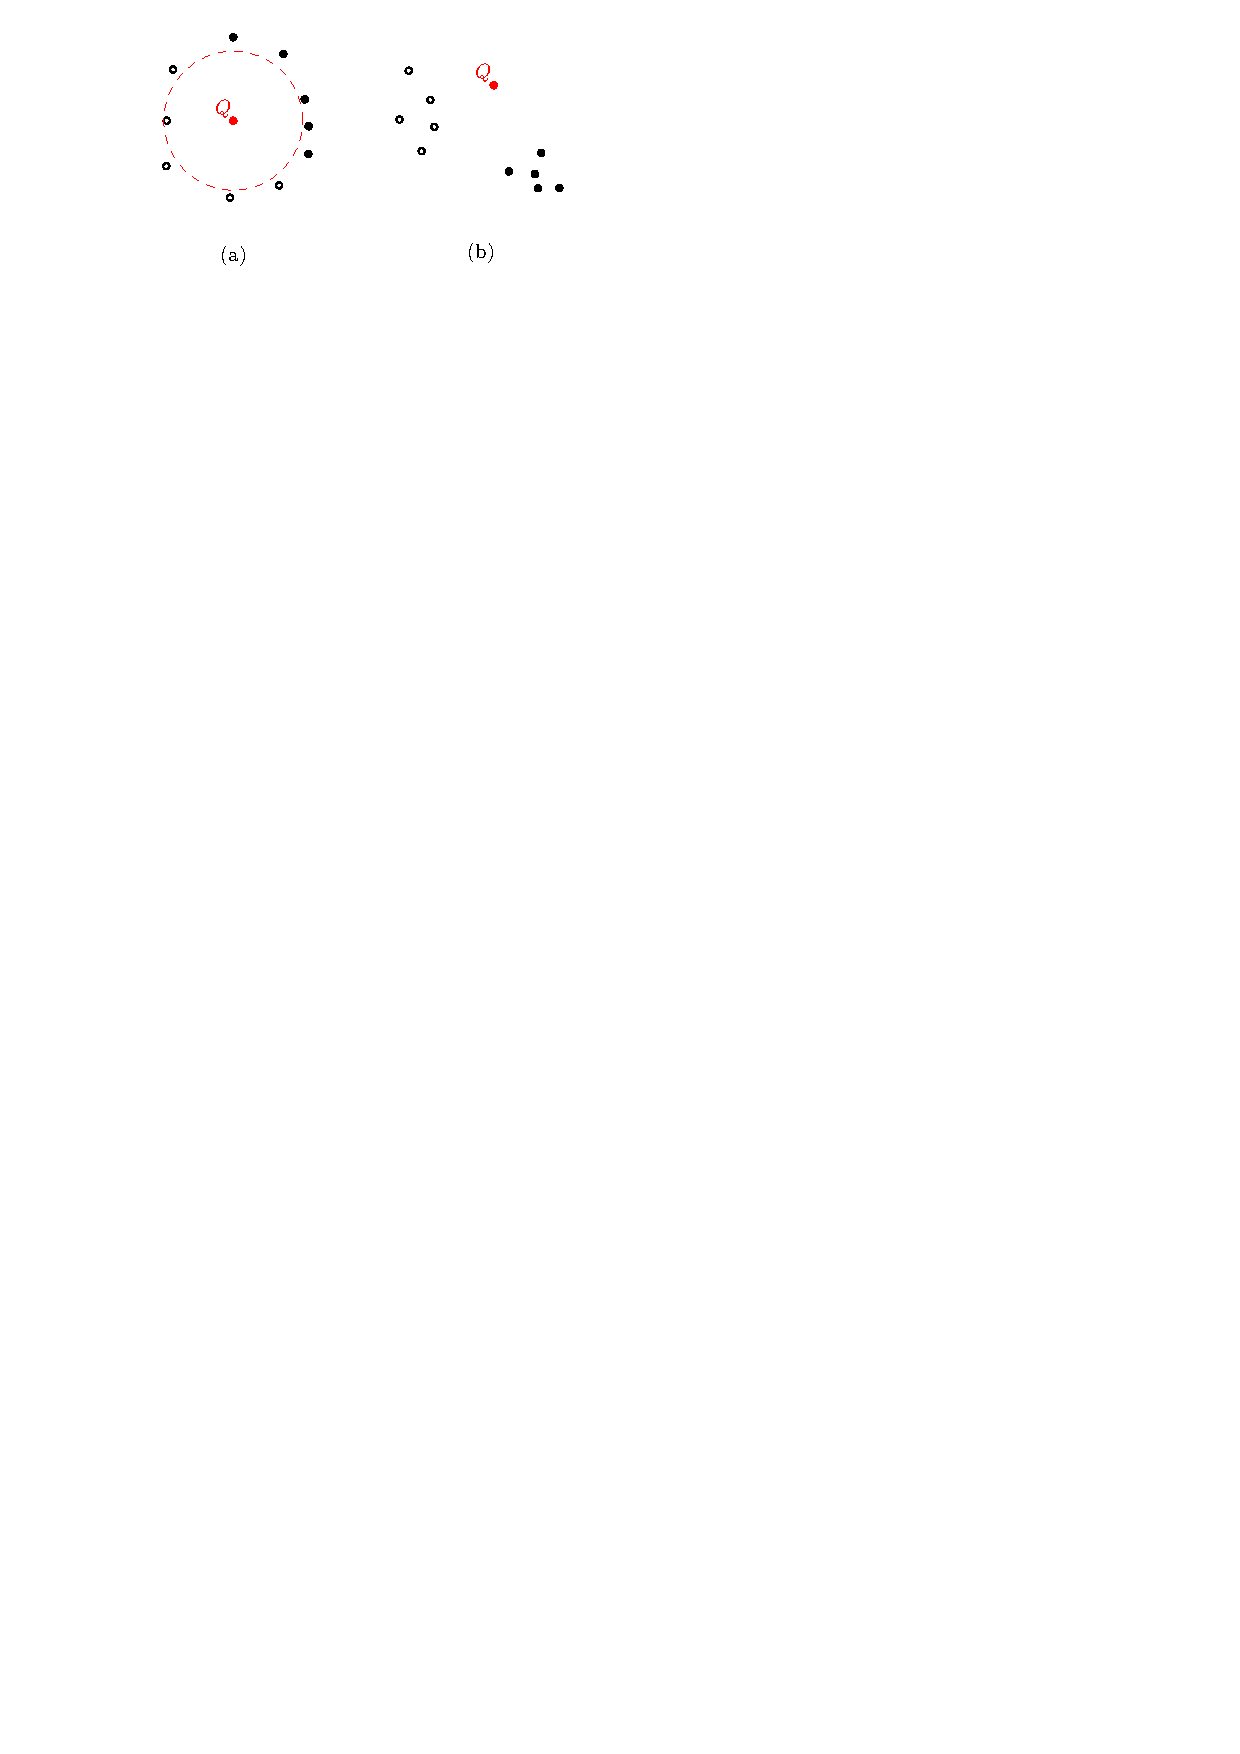
\includegraphics[width=0.7\linewidth]{figs/3/reject.pdf}
  \caption[Two rejection rules used in instance-based learning]{Two rejection rules: (a) ambiguity rejection: $Q$'s estimated collision probability is near $0.5$ or the variance for the estimate is large; (b) distance rejection: when $Q$ is far from all in-collision and collision-free database items.}
  \label{fig:3:reject}
\end{figure}


\subsection{Asymptotic Property of Approximate Collision Query}
\label{subsec:3:knnreasoning:converge}
If the classifier used in the learning-based approximate collision query is effective, we can prove that the collision status returned by the instance-based learning will converge to the exact collision detection results when the size of the dataset increases (asymptotically):
\begin{theorem}
  \label{thm:3:conv}
  The collision query performed using LSH-based $\knn$ will converge to the exact collision detection as the size of the dataset increases.
\end{theorem}
\begin{proof}
We only need to prove that both the probability of a false positive (i.e., returns in-collision status when there is in fact no collision) and a false negative (i.e., returns collision-free when there is in fact a collision) converges to zero, as the size of the database increases.

Given a query, we denote its $r$-neighbor as $B_r$, where $r$ is the distance between the query and its $k$-th nearest neighbor. For a point query, $B_r$ is an $r$-ball around it. For a line query, $B_r$ is the set of all points with distance $r$ to the line (i.e., a line swept-sphere volume). Let $P_1 = \frac{\mu(B_{r(1+\epsilon)} \cap \Cobs)}{\mu(\Cspace)}$ and $P_2 = \frac{\mu(B_{r(1+\epsilon)} \cap \Cfree)}{\mu(\Cspace)}$, which are the probabilities that a uniform sample in $\Cspace$ is in-collision or collision-free and within query's $r(1+\epsilon)$-neighborhood. Here $\mu(\cdot)$ is the volume measure. Let $N$ be the size of the database corresponding to the prior instances.

A false negative occurs if and only if the following two cases are true: 1) there are no in-collision points within $B_{r(1+\epsilon)}$, and therefore the approximate method always returns collision-free; 2) there are in-collision points within $B_{r(1+\epsilon)}$, but the classifier predicts wrong label.

First, we compute the probability for case 1. The event that there are no in-collision points within $B_{r(1+\epsilon)}$ happens either when no dataset point lies within $B_{r(1+\epsilon)}$ or when there exist some points within that ball which are missed due to the approximate nature of LSH-based $\knn$ query. According to Theorem~\ref{thm:3:pplsh}, we have
\begin{align}
  &\ \mathbb P[\text{case 1}] \notag \\
  =&\ \sum_{i=0}^N \binom{N}{i} (1-P_1)^{N-i} P_1^i (1-(1/2 -1/e))^i \notag \\
  =& \ (1-P_1(1/2-1/e))^N \rightarrow 0 \ (\text{as } N \rightarrow \infty). \notag
\end{align}

Case 2 can occur when case 1 does not happen and the classifier gives the wrong results. However, as the classifier is effective, we have
\begin{align}
  &\ \mathbb P[\text{case 2}] \notag \\
 =& \ (1 - \mathbb P[\text{case 1}])\cdot \mathbb P_{\text{error}}[\mathbf x \text{ or } l \text{ in-collision}; \mathcal D] \notag \\
 =& \ (1 - \mathbb P[\text{case 1}])\cdot \mathbb E_{\text{error}}[c(\mathbf x) \text{ or } c(l) \mid \mathcal D] \notag \\
 \rightarrow &\ 0 \ (\text{as } N \rightarrow \infty). \notag
\end{align}

As a result, we have
\begin{equation}
\mathbb P[\text{false negative}] = \mathbb P[\text{case 1}] + \mathbb P[\text{case 2}] \rightarrow 0 \ (\text{as } N \rightarrow \infty) \notag.
\end{equation}

Similarly, a false positive occurs if there are no collision-free points within $B_{r(1+\epsilon)}$ or if there are collision-free points within $B_{r(1+\epsilon)}$ but the classifier still predicts a wrong label. The probability of case 1 can be given as
\begin{equation}
\mathbb P[\text{case 1}] = \ (1-P_2(1/2-1/e))^N \notag
\end{equation}
and the probability of case 2 is
\begin{align}
\mathbb P[\text{case 2}] &= (1 - \mathbb P[\text{case 1}]) \cdot \mathbb P_{\text{error}} [\mathbf x \text{ or } l \text{ collision free}; \mathcal D] \notag \\
 &= (1 - \mathbb P[\text{case 1}])\cdot \mathbb E_{\text{error}}[c(\mathbf x) \text{ or } c(l) \mid \mathcal D]. \notag \\
\end{align}
Both terms converge to zero when the size of the database increases. As a result, we can conclude that the false positive also converges to $0$:
\begin{equation}
\mathbb P[\text{false positive}] = \mathbb P[\text{case 1}] + \mathbb P[\text{case 2}]\rightarrow 0 \ (\text{as } N \rightarrow \infty). \notag
\end{equation}
\end{proof}
%\begin{remark}
%  Note that the convergence of the collision query using LSH-based $\knn$ query is slower than that using the exact $\knn$ based method, whose prediction errors can be given as: $\mathbb P[\text{false negative}] = (1-P_1)^N$ and $\mathbb P[\text{false positive}] \leq (1-P_2)^N$.
%\end{remark}
%
%\begin{remark}
%The fact that the probability of getting false negative (or false positive) converges to $0$ is true if and only if $P_1$ (or $P_2$) is not $0$. Usually we assume that real world obstacles are compact and therefore obstacles in $\Cspace$ are also compact. Thus, if a configuration is collision-free, there is an open set surrounding it that is collision-free as well and therefore $P_2 > 0$. However, a configuration in-collision (i.e., inside a contact set) does not necessarily have a positive $P_1$ (i.e., $P_1$ may be zero). As these kinds of `bad' configurations are of zero measure, our proof of Theorem~\ref{thm:3:conv} still holds.
%\end{remark}


\section{Accelerating Sample-based Planners}
\label{sec:3:planners}

In this section, we first discuss techniques to accelerate various sample-based planners using our learning-based collision query, including 1) how the database is constructed and maintained; 2) how to accelerate various planners; 3) how to handle dynamic environments; 4) how to combine these techniques with non-uniform sampling techniques.
Next, we analyze the factors that can influence the performance of resulting planners using our approximate collision queries. Finally, we prove the completeness and optimality of modified sample-based planners.

\subsection{Database Construction}
When the planner thread starts, the database of prior collision query results is empty. Given a point query, we first compute its $k$-nearest neighboring points $S$. Based on $S$, we check whether distance rejection is necessary. If so, we perform exact collision test and add the query result into the database. Otherwise, we estimate the query's collision probability and the confidence of our estimate, using approaches discussed in Section~\ref{sec:3:knnreasoning}. Next, we check for ambiguity rejection. Based on the outcome of ambiguity rejection, we may again perform exact collision query and add the result to the database; or the estimated collision result can be directly used by a sample-based planner. When a local path query is given, the processing pipeline is similar, except that when performing exact collision checking of the local path, a series of point configurations on the local path are added to the database. In summary, we perform exact collision tests only for queries that are located within regions that are not well covered by the current database D; the resulting query results are added into $\mathcal D$. Later, in Section~\ref{sec:3:planners:planner}, we verify the collision status of a query using exact collision test when it is estimated as collision-free. This test is performed to guarantee the overall motion planning algorithm to be conservative. However, such queries are not added to the database.

Next, we discuss the efficiency of operations on the LSH-based database, which is implemented as a hash table. The hash table starts out empty, so there is no pre-processing overhead. When we decide to add the result for a collision query $\mathbf x$ into the database, we first compute its hashing code $\hat{h}(\mathbf x)$ and then add it into the hash table. This step's complexity remains constant. After warm-up, we begin performing learning-based $\knn$ query on the hash table, which has the complexity $\mathcal O(N^{\rho})$ (all symbols are as defined in Theorem~\ref{thm:3:pllsh}). After adding $N$ items into the hash table and performing $M$ learning-based collision queries, the overall complexity of the database operations becomes $\mathcal O(N + M \cdot N^{\rho})$. Note that the number of all collision queries is larger than $\max(N, M)$; therefore the amortized learning overhead on each collision query is $\mathcal O(1)$.

\subsection{Accelerating Various Planners}
\label{sec:3:planners:planner}


\begin{figure}[htb]
  \subfloat[I-PRM]{\fbox{\begin{minipage}{0.48\linewidth}
      \centering
      \scriptsize
      \label{alg:alg-1}
      \begin{algorithmic}
        \STATE $\texttt{sample}(\mathcal D^{\text{out}}, n)$
        \STATE $V \leftarrow \mathcal D \cap \Cfree$, $E \leftarrow \emptyset$
        \STATE \textbf{foreach} $v \in V$ \textbf{do}
	    \STATE \quad $U \leftarrow \texttt{near}(G^{V, E}, v, \mathcal D^{\text{in}})$
        \STATE \quad \textbf{foreach} $u \in U$ \textbf{do}
	    \STATE \quad \quad \textbf{if} $\texttt{icollide}(v, u, \mathcal D^{\text{in}}) < t$
        \STATE \quad \quad \quad \textbf{if} $\neg \texttt{collide}(v, u, \mathcal D^{\text{out}})$
        \STATE \quad \quad \quad \quad $E \leftarrow E \cup (v,u)$
        \STATE
        \STATE \texttt{near}: nearest neighbor search.
        \STATE \texttt{icollide}: probabilistic collision checking based on $\knn$.
        \STATE \texttt{collide}: exact local path collision checking.
        \STATE $\mathcal D^{\text{in/out}}$: prior instances as input/output.
      \end{algorithmic}
  \end{minipage}}}
  \subfloat[I-lazyPRM]{\fbox{\begin{minipage}{0.48\linewidth}
      \centering
      \scriptsize
      \label{alg:alg-2}
      \begin{algorithmic}
        \STATE $\texttt{sample}(\mathcal D^{\text{out}}, n)$
        \STATE $V \leftarrow \mathcal D \cap \Cfree$, $E \leftarrow \emptyset$
        \STATE \textbf{foreach} $v \in V$ \textbf{do}
	    \STATE \quad $U \leftarrow \texttt{near}(G^{V, E}, v, \mathcal D^{\text{in}}) \{v\}$
        \STATE \quad \textbf{foreach} $u \in U$ \textbf{do}
        \STATE \quad \quad $w \leftarrow \texttt{icollide}(v, u, \mathcal D^{\text{in}})$
	    \STATE \quad \quad $l \leftarrow \|(v, u)\|$
        \STATE \quad \quad $E \leftarrow E \cup (v, u)^{w, l}$
        \STATE \quad \textbf{do}
        \STATE \quad \quad search path $p$ on $G(V, E)$ which minimizes
	    \STATE \quad \quad \quad $\sum_{e} l(e) + \lambda \min_{e} w(e)$.
        \STATE \quad \quad \textbf{foreach} $e \in p$, \texttt{collide}$(e, \mathcal D^{\text{out}})$
        \STATE \quad \textbf{while} $p$ not valid
      \end{algorithmic}
  \end{minipage}}}
  \\
  \subfloat[I-RRT]{\fbox{\begin{minipage}{0.48\linewidth}
      \centering
      \scriptsize
      \label{alg:alg-3}
      \begin{algorithmic}
        \STATE $V, \mathcal D \leftarrow x_{\text{init}}$, $E \leftarrow \emptyset$
	    \STATE \textbf{while} $x_{\text{goal}}$ not reach
        \STATE \quad $x_{\text{rnd}} \leftarrow \texttt{sample-free}(\mathcal D^{\text{out}}, 1)$
        \STATE \quad $x_{\text{nst}} \leftarrow \texttt{inearst}(G^{V,E}, x_{\text{rnd}}, \mathcal D^{\text{in}})$
        \STATE \quad $x_{\text{new}} \leftarrow \texttt{isteer}(x_{\text{nst}}, x_{\text{rnd}}, \mathcal D^{\text{in}, \text{out}})$
        \STATE \quad \textbf{if} $\texttt{icollide}(x_{\text{nst}}, x_{\text{new}}) < t$
        \STATE \quad \quad \textbf{if} $\neg \texttt{collide}(x_{\text{nst}}, x_{\text{new}})$
        \STATE \quad \quad \quad $V \leftarrow V \cup x_{\text{new}}$, $E \leftarrow E \cup (x_{\text{new}}, x_{\text{nst}})$
        \STATE
        \STATE \texttt{inearest}: find the nearest tree node that is long and has high collision-free probability.
        \STATE \texttt{isteer}: steer from a tree node to a new node, using \texttt{icollide} for validity checking.
        \STATE \texttt{rewire}: RRT${}^*$ routine used to update the tree topology for optimality guarantee.
      \end{algorithmic}
  \end{minipage}}}
  \subfloat[I-RRT${}^*$]{\fbox{\begin{minipage}{0.48\linewidth}
      \centering
      \scriptsize
      \label{alg:alg-4}
      \begin{algorithmic}
        \STATE $V, \mathcal D \leftarrow x_{\text{init}}$, $E \leftarrow \emptyset$
	    \STATE \textbf{while} $x_{\text{goal}}$ not reach
        \STATE \quad $x_{\text{rnd}} \leftarrow \texttt{sample-free}(\mathcal D^{\text{out}}, 1)$
        \STATE \quad $x_{\text{nst}} \leftarrow \texttt{inearst}(G^{V,E}, x_{\text{rnd}}, \mathcal D^{\text{in}})$
        \STATE \quad $x_{\text{new}} \leftarrow \texttt{isteer}(x_{\text{nst}}, x_{\text{rnd}}, \mathcal D^{\text{in}, \text{out}})$
        \STATE \quad \textbf{if} $\texttt{icollide}(x_{\text{nst}}, x_{\text{new}}) < t$
        \STATE \quad \quad \textbf{if} $\neg \texttt{collide}(x_{\text{nst}}, x_{\text{new}})$
        \STATE \quad \quad \quad $V \leftarrow V \cup x_{\text{new}}$
        \STATE \quad \quad \quad $U \leftarrow \texttt{near}(G^{V,E}, x_{new})$
        \STATE \quad \quad \quad \textbf{foreach} $x \in U$, compute weight $c(x) = $
        \STATE \quad \quad \quad \quad $\lambda \|(x, x_{\text{new}})\|+ \texttt{icollide}(x, x_{\text{new}}, \mathcal D^{\text{in}})$
        \STATE \quad \quad \quad sort $U$ according to weight $c$.
        \STATE \quad \quad \quad Let $x_{\text{min}}$ be the first $x \in U$ with $\neg \texttt{collide}(x, x_{\text{new}})$
        \STATE \quad \quad \quad $E \leftarrow E \cup (x_{\text{min}}, x_{\text{new}})$
        \STATE \quad \quad \quad \textbf{foreach} $x \in U$, \texttt{rewire}$(x)$
      \end{algorithmic}
  \end{minipage}}}
  \caption[Instance-based learning framework can be easily integrated with different motion planners]{Instance-based learning framework can improve different motion planners. Here we present four modified planners.}
  \label{fig:3:planners}
\end{figure}



Algorithm~\ref{algo:3:collisionquery} illustrates our basic approach to apply the learning framework: we use the computed collision probability as a filter to reduce the number of exact collision queries. If a given configuration or local path query is close to in-collision instances, then it has a high probability of being in-collision. Similarly, if a query has many collision-free instances around it, it is likely to be collision-free. In our implementation, we cull away only those queries with high collision probabilities. For queries with high collision-free probability, we still perform exact collision tests on them in order to guarantee that the overall collision detection algorithm is conservative.
In Figure~\ref{fig:3:planners}(a), we show how our probabilistic culling strategy can be integrated with the PRM algorithm by only performing exact collision checking (\texttt{collide}) for queries with collision probability (\texttt{icollide}) larger than a given threshold $t$.
Note that the neighborhood search routine (\texttt{near}) can use LSH-based point-point $\knn$ query. \texttt{icollide} is computed according to Equation~\ref{eq:3:knnclassifier} or Equation~\ref{eq:3:knnclassifierline}.

In Figure~\ref{fig:3:planners}(b), we show how to use the collision probability as a cost function with the lazyPRM algorithm~\cite{Kavraki96}. In the basic version of lazyPRM algorithm, the expensive local path collision checking is delayed till the search phase. The basic idea is that the algorithm repeatedly searches the roadmap to compute the shortest path between the initial and goal nodes, performs collision checking along the edges, and removes the in-collision edges from the roadmap. However, the shortest path usually does not correspond to a collision-free path, especially in complex environments. We improve the lazyPRM planner using learning-based collision queries. We compute the collision probability for each roadmap edge during roadmap construction, based on Equation~\ref{eq:3:linepointprob}. The probability ($w$) as well as the length of the edge ($l$) are stored as costs of the edge. During the search step, we try to compute the shortest path with a minimum collision probability, i.e., a path that minimizes the cost $\sum_{e} l(e) + \lambda \min_{e} w(e)$, where $\lambda$ is a parameter that controls the relative weight of path length and collision probability. As the prior knowledge about obstacles is implicitly taken into account based on collision probability, the resulting path is more likely to be collision-free.

Finally, the collision probability can be used by the motion planner to explore $\Cfree$ in an efficient manner. We use RRT to illustrate this benefit (Figure~\ref{fig:3:planners}(c)). Given a random sample $x_{\text{rnd}}$, RRT computes a node $x_{\text{nst}}$ among the prior collision-free configurations that are closest to $x_{\text{rnd}}$ and expands from $x_{\text{nst}}$ towards $x_{\text{rnd}}$. If there is no obstacle in $\Cspace$, this exploration technique is based on the Voronoi heuristic that biases the planner towards the unexplored regions. However, the existence of obstacles affects its performance: the planner may run into $\Cobs$ shortly after expansion, and the resulting exploration is limited. Using instance-based learning, we can estimate the collision probability for local paths connecting $x_{\text{rnd}}$ with each of its neighbors and choose $x_{\text{nst}}$ as the one with both a long edge length and a small collision probability (i.e., $x_{\text{nst}} = \argmax(l(e) - \lambda \cdot w(e))$, where $\lambda$ is a parameter used to control the relative weight of these two terms). A similar strategy can also be used for RRT${}^*$, as shown in Figure~\ref{fig:3:planners}(d).




\subsection{Narrow Passages and Non-uniform Samples}
\label{subsec:3:narrowpassage}
Narrow passages are a key problem for sample-based motion planners. In general, it is difficult to generate enough number of samples in the narrow passages and capture the connectivity of the free space. Narrow passages can lead to some additional issues in terms of the learning-based collision status classifier presented in Section\ref{subsec:3:knnreasoning:pointclassifier}. In narrow passages, a collision-free query point configuration can be wrongly classified as in-collision.% as shown in Figure~\ref{fig:3:narrowpassage}.
This is because the learning algorithm assumes the spatial coherency about the collision status, i.e., nearby samples in the $\Cspace$ tend to have the same collision status. However, such spatial coherency may not work in the regions around narrow passages and this may reduce the accuracy of collision status estimated via the learning algorithm. This reduced accuracy can also decrease the performance of the planner in narrow passages. If a random planner can indeed generate a free-space sample in the narrow passage, the learning algorithm may incorrectly classify it as in-collision and may not add it to the database $\mathcal D$ and the roadmap/tree-structure used by the planner. As a result, the planner may not be able to capture the connectivity of the space correctly around that narrow passage.


One solution to the above problem is to verify a query's collision status occasionally using exact collision test, even when the learning algorithm estimates the query to have a large collision probability. In particular, suppose the estimated collision probability of a query is $p$, where $p \in (0.5, 1]$, then with a probability of $\max(1 - p, p_s)$, we check the exact collision status of the query, where $p_s$ is a small value (e.g., $0.01$).

The non-uniform sampling strategies used in different sample-based planners~\cite{Boor:1999:ICRA,Rodriguez:2006,Zheng:2005} can be combined with our learning based collision query to generate more narrow passage samples in the database $\mathcal D$ and the planner's roadmap. The samples generated using these strategies are directly added into the database and are used later by the learning algorithm.


\subsection{Performance Analysis}

The learning-based planners are faster, mainly because we replace some of the expensive, exact collision queries with relatively cheap $\knn$ queries. Let the timing cost for a single exact collision query be $T_C$ and for a single $\knn$ query be $T_K$, where $T_K < T_C$. Suppose the original planner performs $C_1$ collision queries and the instance-based learning enhanced planners performs $C_2$ collision queries and $C_1 - C_2$ $\knn$ queries, where $C_2 < C_1$. We also assume that the two planners spend the same time $A$ on other computations within a planner, such as sample generation, maintaining the roadmap or the tree structure, etc. Then the speedup ratio obtained by learning-based planner is:
\begin{equation}
  R = \frac{T_C \cdot C_1 + A}{T_C \cdot C_2 + T_K \cdot (C_2 - C_1) + A}.
\end{equation}
Therefore, if $T_C \gg T_K$ and $T_C \cdot C_1 \gg A$, we have $R \approx C_1 / C_2$, i.e., if the higher number of exact collision queries are culled, we can obtain a higher speedup. The extreme speedup ratio $C_1 / C_2$ may not be reached, however, for two reasons. 1) $T_C \cdot C_1 \gg A$ may not hold, such as when the underlying collision-free path solution lies in some narrow passages ($A$ is large) or in open spaces ($T_C \cdot C_1$ is small); or 2) $T_C \gg T_K$ may not hold, such as when the environment and robot have low geometric complexity (i.e., $T_C$ is small) or the instance dataset is large and the cost of the resulting $\knn$ query is high (i.e., $T_K$ is large).

Note that $R$ is only an approximation of the actual acceleration ratio. It may overestimate the speedup, because a collision-free local path may have a collision probability higher than a given threshold; our learning-based collision approach filters such high probabilities out. If such a collision-free local path is critical for
the connectivity of the roadmap, such false positives due to instance-based learning will cause the resulting planner to perform more exploration, and thereby increases the overall planning time. As a result, we need to choose an appropriate threshold that can provide a balance: we need a large threshold to filter out more collision queries and increase $R$; at the same time, we need to use a small threshold to reduce the number of false positives. However, the threshold choice is not important in the asymptotic sense. According to Theorem~\ref{thm:3:conv}, the false positive error converges to $0$ when the database size increases.

$R$ may also underestimate the actual speedup, because the timing cost for different collision queries can be different. For configurations near the boundary of $\Cobs$, the collision queries are more expensive. Therefore, the timing cost of checking the collision status for an in-collision local path is usually larger than that of checking a collision-free local path, because the former always has one configuration on the boundary of $\Cobs$. As a result, it is possible to obtain a speedup larger than $C_1 / C_2$.

\subsection{Completeness and Optimality}
As a natural consequence of Theorem~\ref{thm:3:conv}, we can prove the probabilistic completeness and optimality of the new planners. To avoid the narrow passage problems, in this theorem, we assume that the new planners apply the heuristics mentioned in Section~\ref{subsec:3:narrowpassage}. In other words, we assume $p_s > 0$ in order to guarantee that the critical samples in the narrow passage will not be filtered out by mistake.
\begin{theorem}
  \label{thm:3:complete}
  I-PRM, I-lazyPRM, I-RRT are probabilistically complete. I-RRT${}^*$ is probabilistically complete and asymptotically optimal.
\end{theorem}
\begin{proof}
  A motion planner MP is probabilistically complete if its failure probability, i.e., when a collision-free path exists, the probability that it cannot find a solution after $N$ samples converges to $0$ when the number of samples $N$ increases: $\lim_{N\rightarrow \infty}\mathbb P [\text{MP fails}] = 0$, where \mbox{$[$MP fails$]$} denotes the event that the motion planner fails to find a solution after $N$ samples, when the solution exists.

  Suppose we replace MP's exact collision detection query by the learning-based query and denote the new planner as I-MP. I-MP can fail in two cases: 1) MP fails; 2) MP computes a solution but some edges on the collision-free path are classified as in-collision by our learning algorithm (i.e., false positives). Let $L$ be the number of edges in the solution path and let $E_i$ denote the event that the $i$-th edge is incorrectly classified as in-collision. As a result, we have
  \begin{equation}
    \begin{aligned}
      & \ \mathbb P [\text{I-MP fails}] \\
      =& \ \mathbb P [\text{MP fails}] + (1 - \mathbb P [\text{MP fails}]) \cdot \mathbb P[\bigcup_{i=1}^L E_i] \\
      \leq& \ \mathbb P [\text{MP fails}] + \sum_{i=1}^L \mathbb P[E_i].
    \end{aligned}
  \end{equation}
  Similar to \mbox{$[$MP fails$]$}, the event \mbox{$[$I-MP fails$]$} denotes the event that the new motion planner fails to find a solution after $N$ samples, when the solution exists.
  According to Theorem~\ref{thm:3:conv}, $\lim_{N\rightarrow \infty}\mathbb P [E_i] = 0$ and $L$ is a finite number, then we have $\lim_{N\rightarrow \infty}\mathbb P [\text{I-MP fails}] = 0$, i.e., I-MP is probabilistically complete. Therefore, as PRM, lazyPRM, RRT and RRT${}^*$ are all probabilistically complete, we can prove that I-PRM, I-lazyPRM, I-RRT and  I-RRT${}^*$ are all probabilistically complete.

  Similarly, if MP is asymptotically optimal, then I-MP may not converge to the optimal path only when some of the path edges are classified as in-collision by the learning algorithm and this probability converges to zero. As a result, I-RRT${}^*$ is asymptotically optimal.
\end{proof}



\section{Results and Discussions}
\label{sec:3:results}
In this section, we evaluate the performance of our new planners. Figure~\ref{fig:3:benchmark} and Figure~\ref{fig:3:benchmark2} show the articulated PR2 and rigid body benchmarks we used to evaluate the performance. We evaluate each planner on different benchmarks. For each combination of planner and benchmark we ran $50$ instances of the planner, and computed the average planning time as an estimate of the planner's performance on this benchmark. The algorithm is implemented in C++ and all the experiments are performed on a PC with an Intel Core i7 3.2GHz CPU with 2GB memory. The exact collision tests are performed using FCL collision library~\cite{Pan:ICRA:2012}.

\subsection{Pipeline and Results}

The learning-based planners use a `cold start', i.e., they start with an empty database of prior collision query results, which means that they have no knowledge about the environment in the beginning. As a result, during the first few queries performed by sample-based planner, the learning-based collision framework will find that it does not have sufficient information to predict the collision status of a given configuration or a local path. In these cases,we land up using exact collision checking algorithms. During this phase, the learning-based planner will behave exactly the same as the original planner, except that the results from exact collision queries will be stored in the database. This process is called the `warm up' of the instance-based learning framework. After several planning queries, there will be enough information in the database about $\Cspace$ to perform learning, and the acceleration brought by the learning method begins to counteract its overhead during the following queries.

The comparison results are shown in Table~\ref{tab:3:compare} and Table~\ref{tab:3:compare2}, corresponding to PR2 benchmarks and rigid body benchmarks, respectively. Based on these benchmarks, we observe that:
\begin{itemize}
\item The learning-based planners provide more speedup on articulated models. Exact collision checking on articulated models is more expensive than exact collision checking on rigid models, because for articulated models we need to compute self-collision as well as check for collisions between each component of the body and each obstacle in the environment. This makes $T_C$ larger and results in larger speedups.
\item The speedup of I-PRM over PRM is relatively large, since exact collision checking takes a significant fraction of overall time within PRM algorithm. I-lazyPRM also provides good speedup as the candidate path is nearly collision-free and can greatly reduce the number of exact collision queries in lazy planners. The speedups of I-RRT and I-RRT${}^*$ are limited or can even be slower than the original planners, especially on simple rigid body benchmarks. This is because the original planners are already quite efficient on simple benchmarks, and instance-based learning can result in some overhead.
\end{itemize}


We also analyze the accuracy of our learning-based collision status estimation algorithm in Figure~\ref{fig:3:accuracy}. For databases of different sizes, we compute the average learning accuracy on $100$ point queries or local path queries. If an ambiguity rejection or a distance rejection happens for a query, we measure the learning accuracy for this query as $0.5$ because any estimate is no better than random guess, and we in fact perform exact collision checking on such samples. This explains why the learning accuracy is $0.5$ when the database is empty. From the result, we can see the learning accuracy increases when the database becomes larger.


As the learning-based planners use a `cold start', we need to point out that the acceleration results shown in Table~\ref{tab:3:compare} and Table~\ref{tab:3:compare2} show only part of the speedups that can be obtained using a learning-based framework. As more collision queries are performed and their results are stored in the dataset, the resulting planner has more information about $\Cobs$ and $\Cfree$, and becomes more efficient in terms of culling. Ideally, we can filter out all in-collision queries and obtain a high speedup. In practice, we do not achieve ideal speedups due to two reasons: 1) we only have a limited number of samples in the dataset; 2) the overhead of the $\knn$ query increases as the dataset size increases. As a result, when we perform the global motion planning computation repeatedly, the planning time will first decrease to a minimum, and then increase. This phenomenon is shown in Figure~\ref{fig:3:curve}. To avoid such problem, we monitor the average planning time of the most recent planning queries, and to stop adding new data into the database when the average planning time starts to increase. The result of this strategy is shown in Figure~\ref{fig:3:curve2}. In practice, the memory consumed by our modified motion planners is about 2-3 times more (due to the database) than the original planners.

\begin{figure}[t]
  \centering
  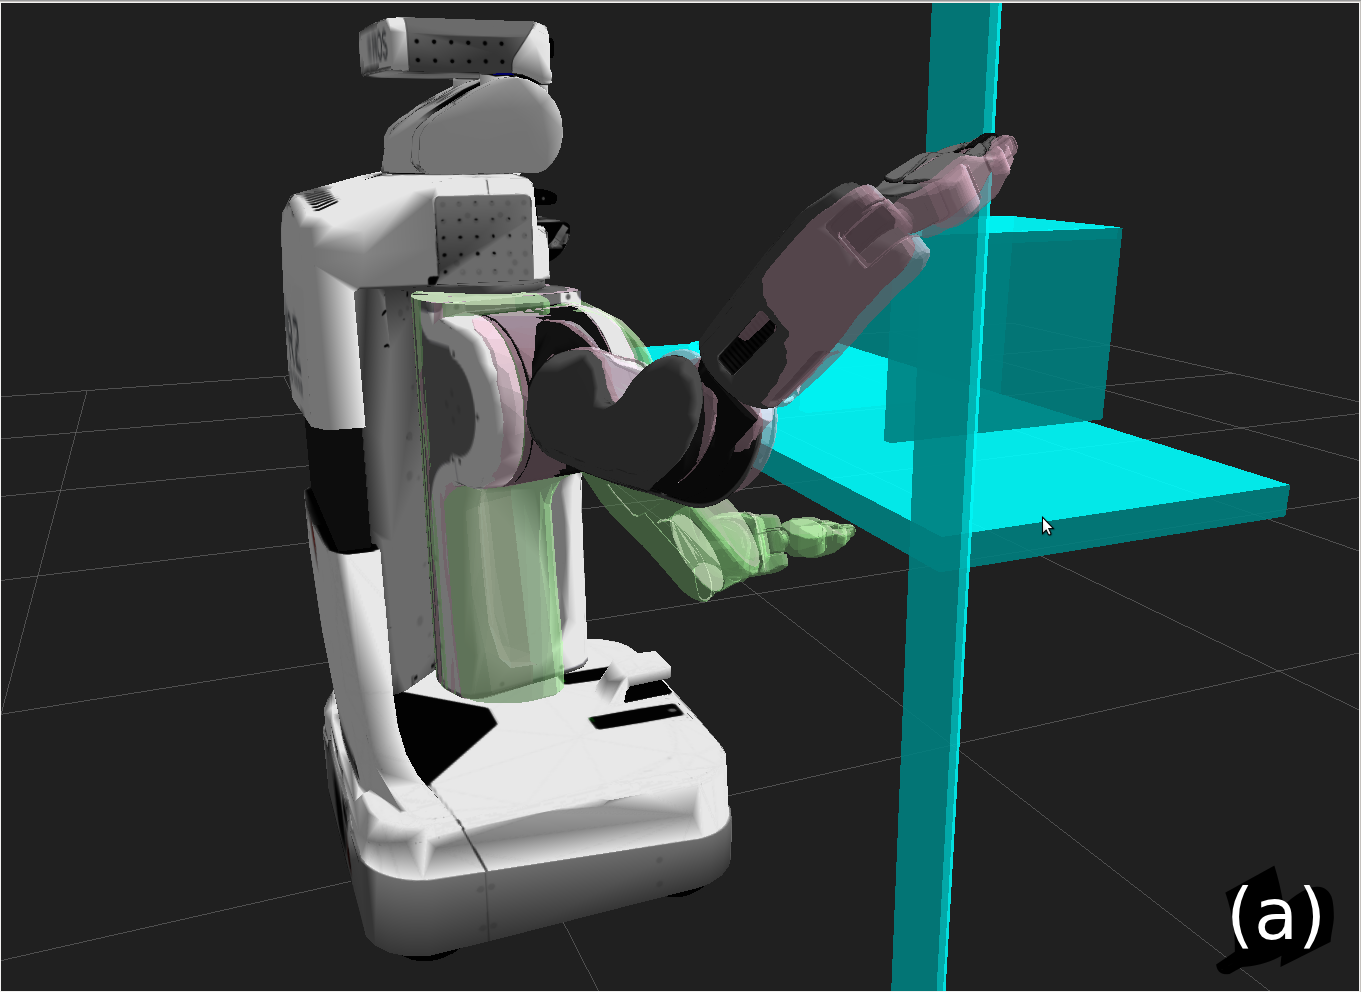
\includegraphics[width=0.24\linewidth]{figs/3/benchmark1.png}
  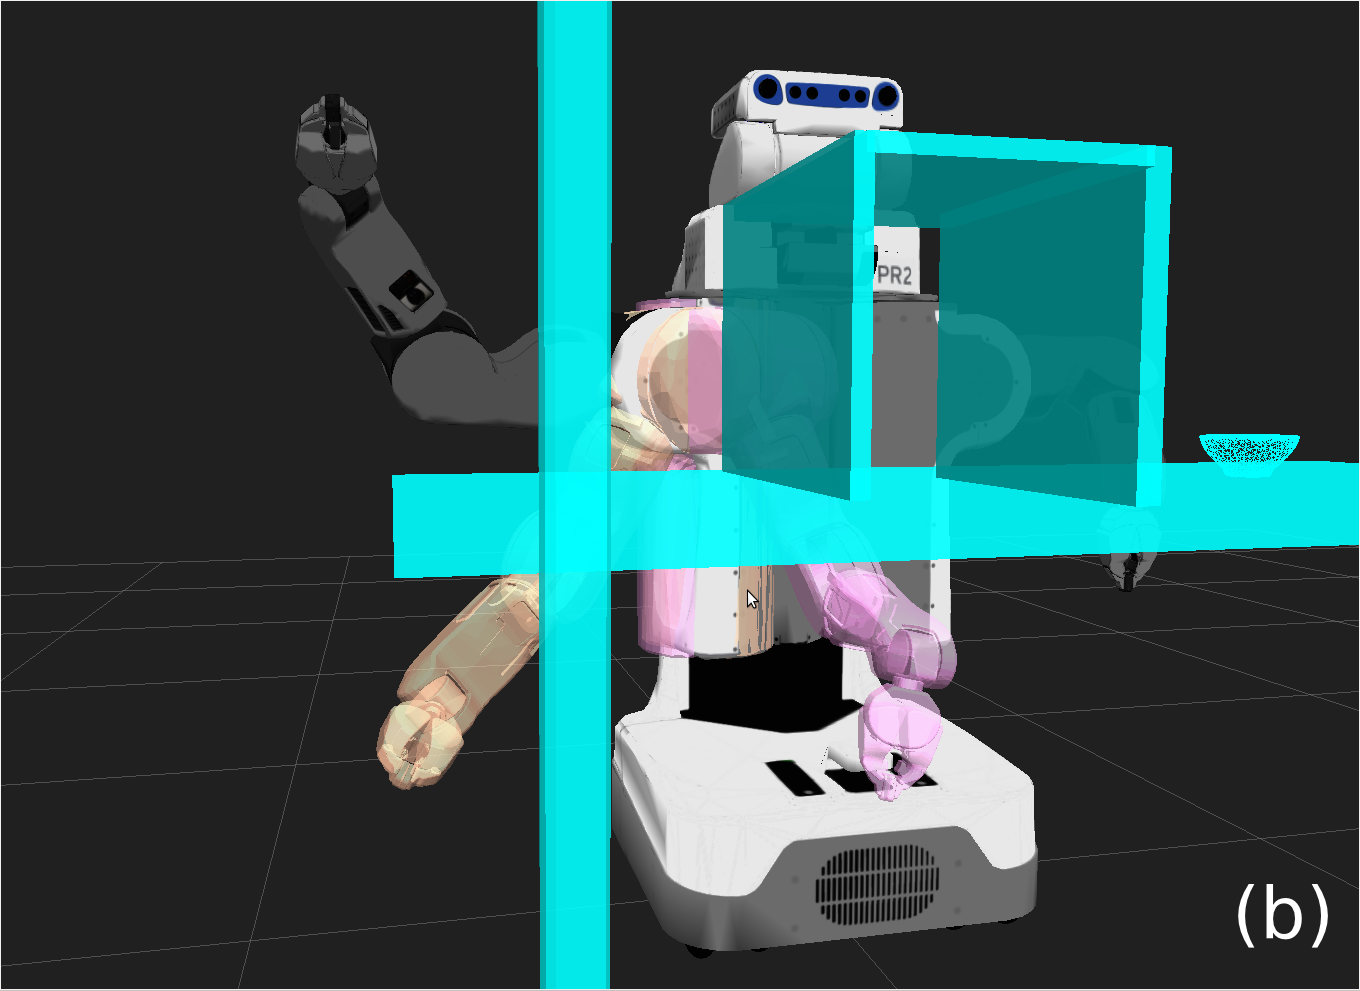
\includegraphics[width=0.24\linewidth]{figs/3/benchmark2.png}
  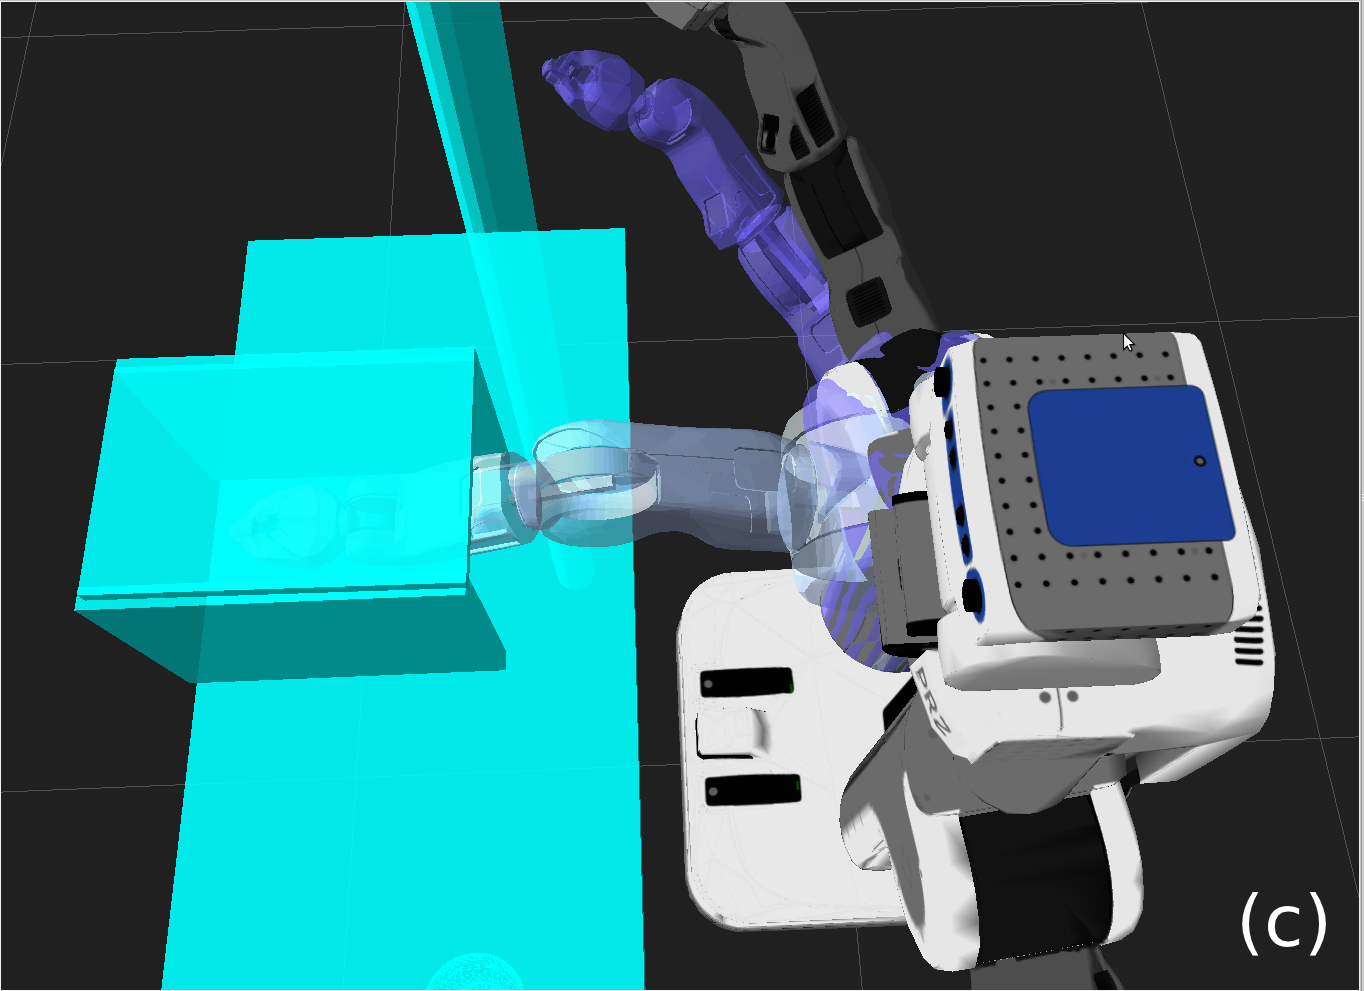
\includegraphics[width=0.24\linewidth]{figs/3/benchmark3.png}
  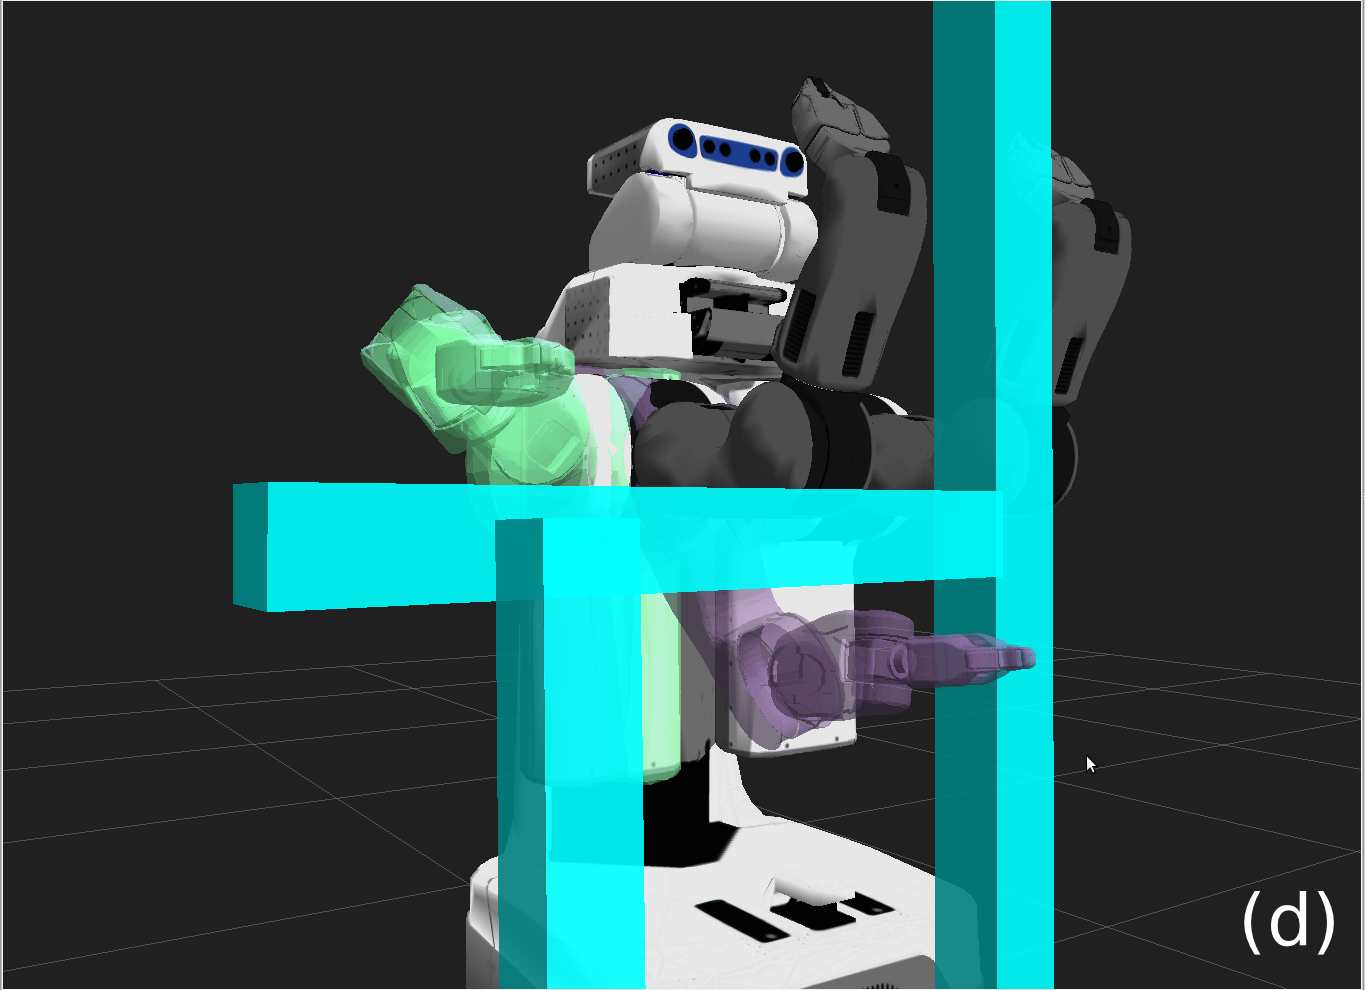
\includegraphics[width=0.24\linewidth]{figs/3/benchmark4.png}
  \caption[PR2 planning benchmarks for instance-based learning]{\label{fig:3:benchmark} PR2 planning benchmarks: robot arms with different colors show the initial and goal configurations. The first three benchmarks are of the same environment, but the robot's arm is in different places: (a) moves arm from under desk to above desk; (b) moves arm from under desk to another position under desk; and (c) moves arm from inside the box to outside the box. In the final benchmark, the robot tries to move arm from under a shelf to above it. The difficulty order of the four benchmarks is (c) $>$ (d) $>$ (b) $>$ (a). These planning problems are for PR2's $7$-DOF robot arm.}
\end{figure}

\begin{figure}[t]
  \centering
  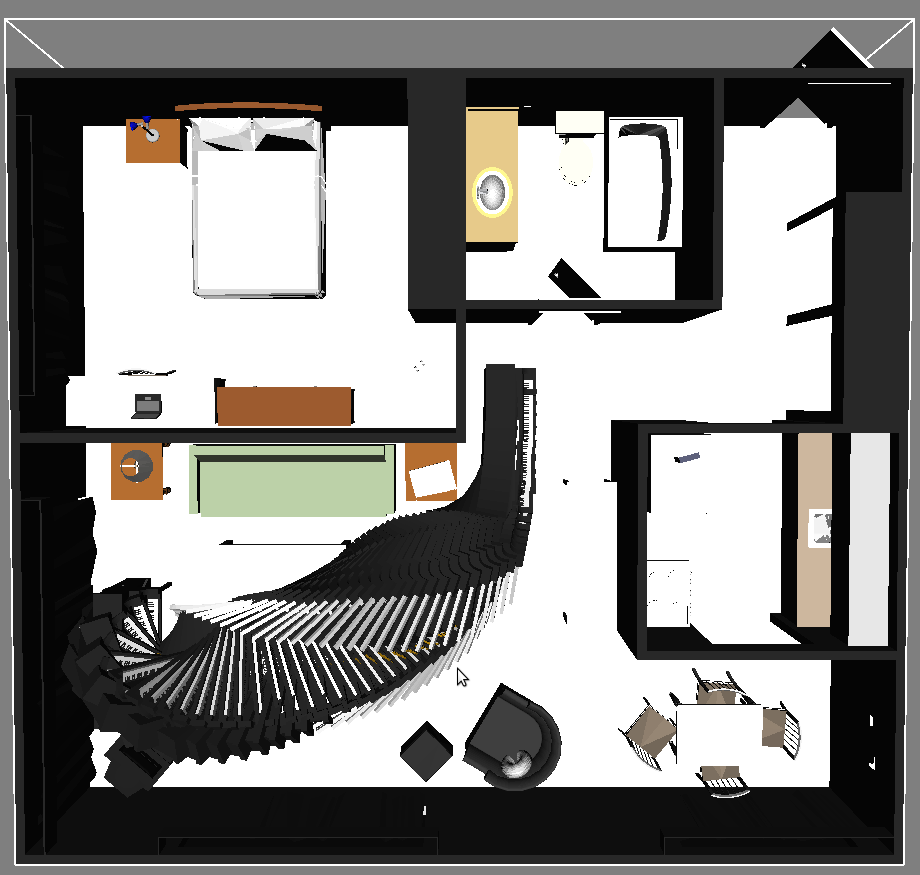
\includegraphics[width=0.180\linewidth]{figs/3/apartment.png}
  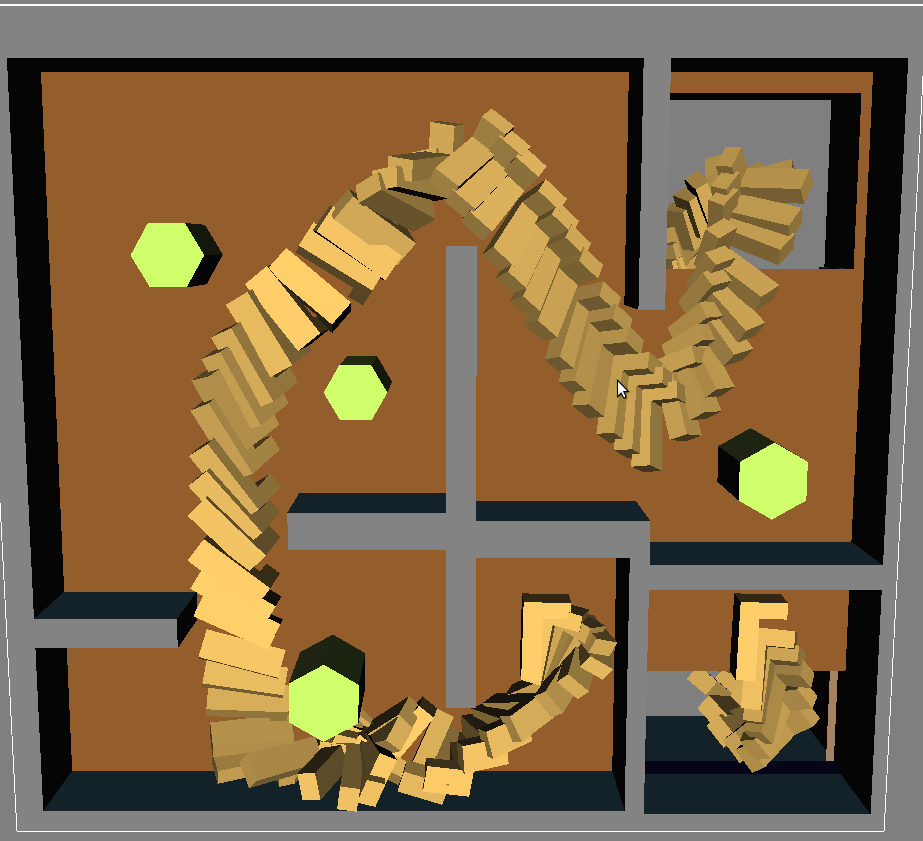
\includegraphics[width=0.188\linewidth]{figs/3/cubicles.png}
  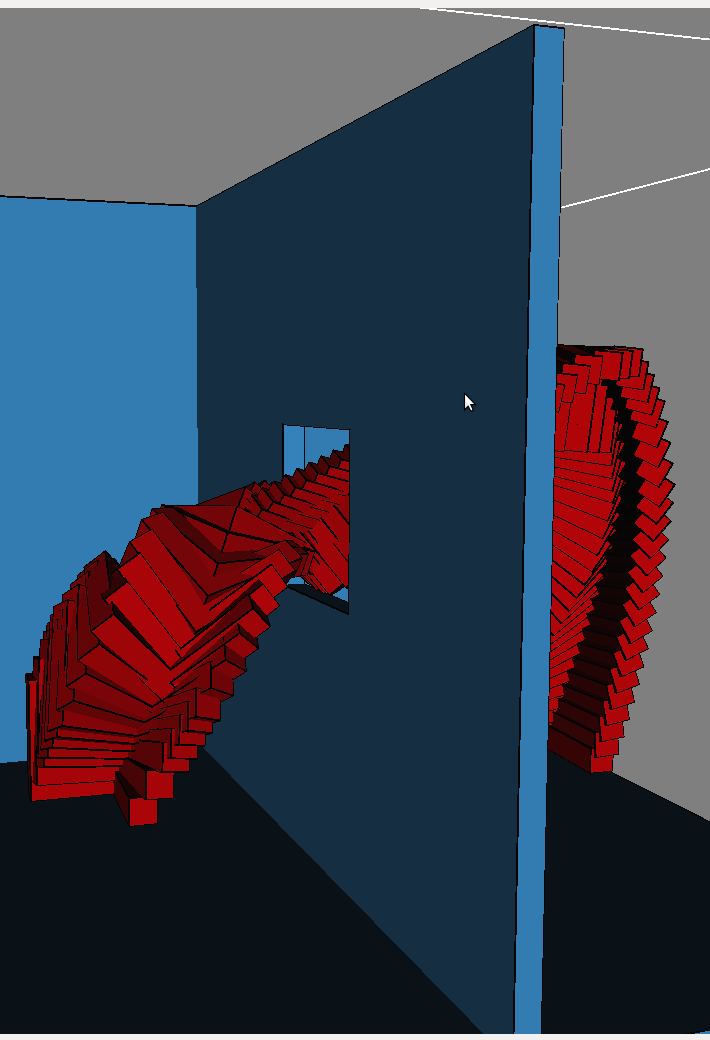
\includegraphics[width=0.118\linewidth]{figs/3/easy.png}
  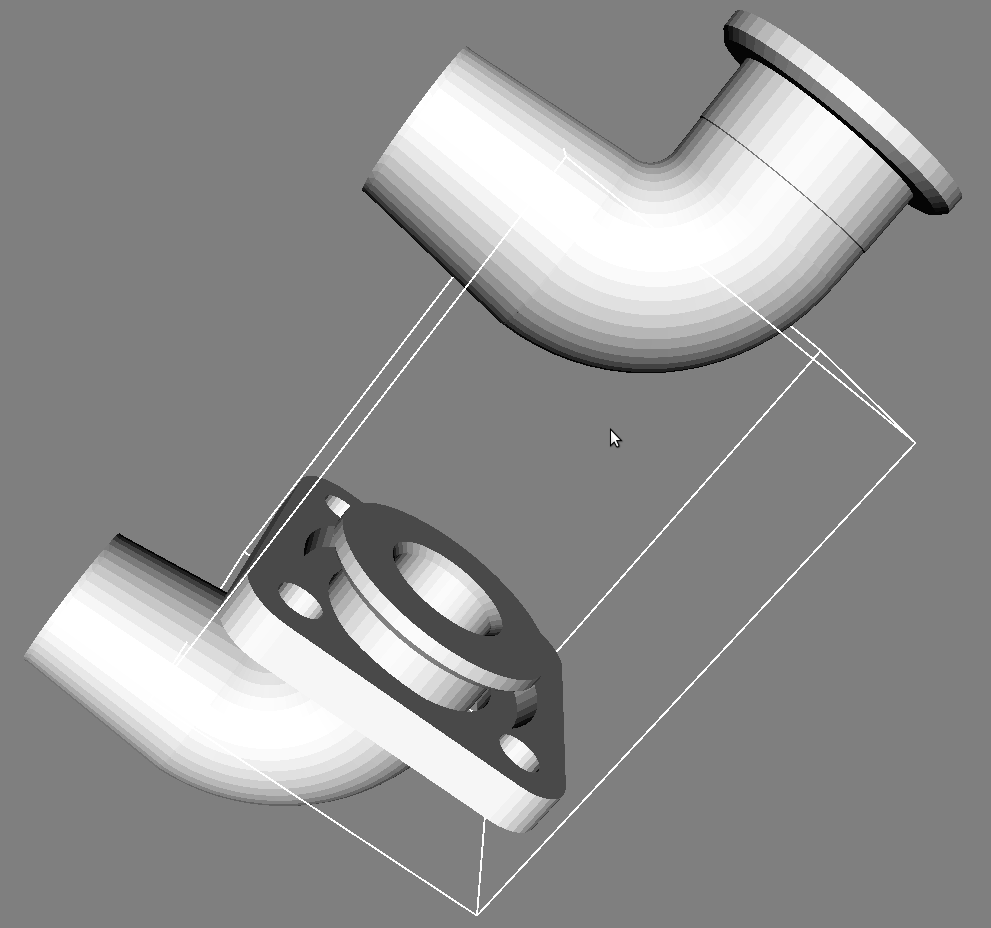
\includegraphics[width=0.184\linewidth]{figs/3/flange.png}
  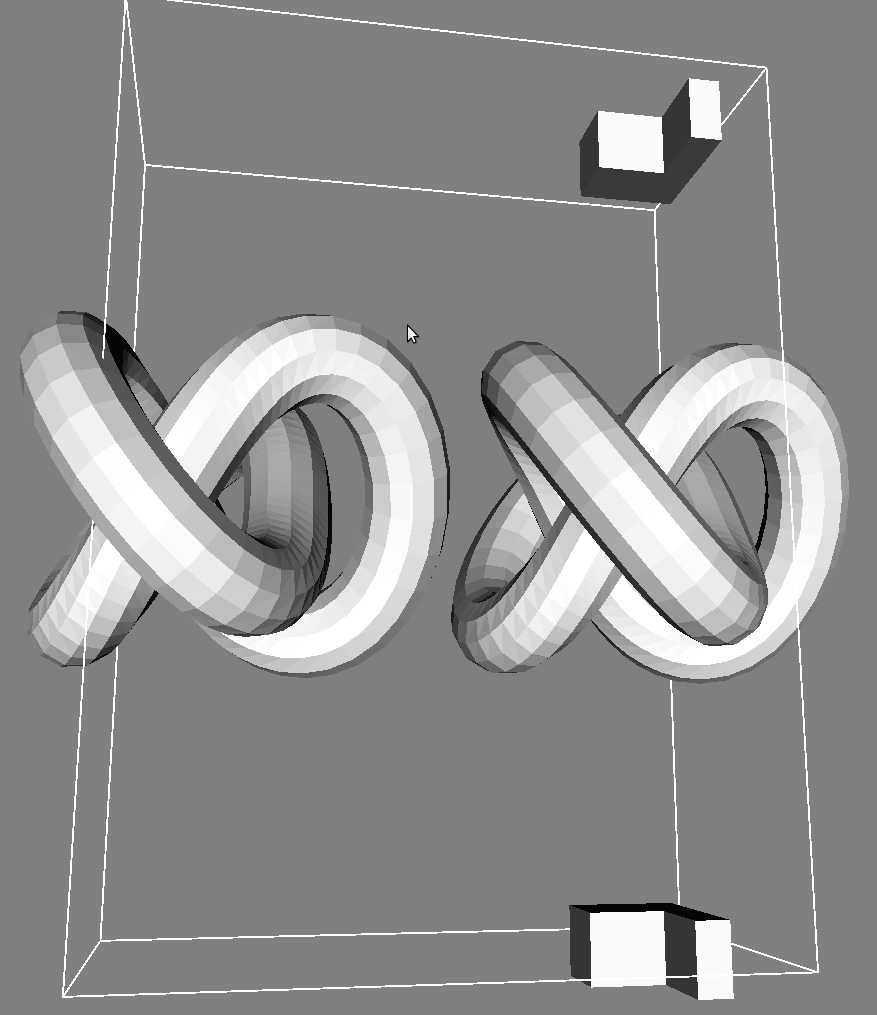
\includegraphics[width=0.150\linewidth]{figs/3/torus.png}
  \caption[Rigid body planning benchmarks for instance-based learning]{\label{fig:3:benchmark2} Rigid body planning benchmarks: from left to right, apartment, cubicles, easy, flange and torus. Apartment benchmark tries to move the piano to the hallway near the door entrance; in cubicles benchmark, the robot moves through a simple office-like environment where the robot needs to fly through the basement; both flange and torus benchmarks contain a narrow passage. These problems are with $6$ DOFs. }
\end{figure}


\begin{figure}[t]
  \centering
  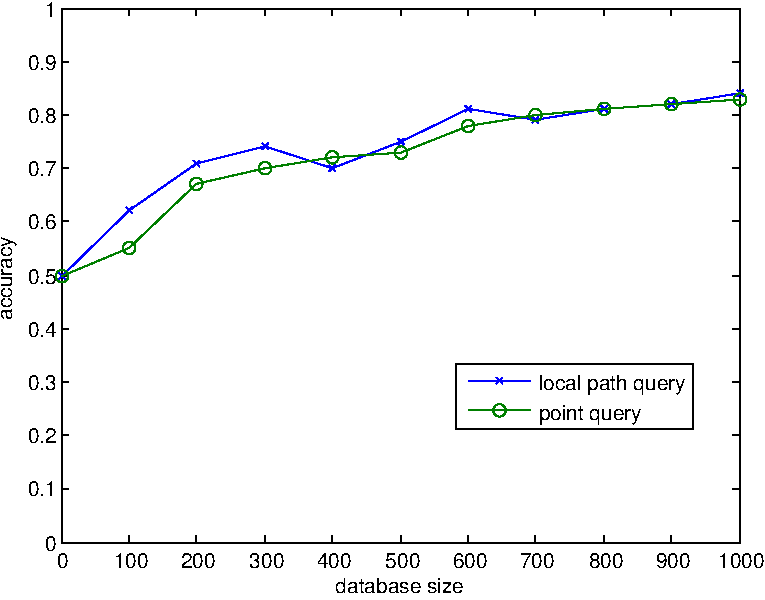
\includegraphics[width=0.8\linewidth]{figs/3/accuracy-crop.pdf}
  \caption[Accuracy of instance-based learning framework on various benchmarks.]{\label{fig:3:accuracy} The accuracy result for benchmark shown in Figure~\ref{fig:3:benchmark}(a). For databases of different sizes, we compute the average accuracy on $100$ point queries or local path queries. If an ambiguity rejection or a distance rejection happens for a query, we measure its accuracy as $0.5$ because any estimate is no better than random guess, and we in fact perform exact collision checking on such samples. This is why the accuracy is $0.5$ when the database is empty.}
\end{figure}




\begin{table}[htb]
\begin{center}
\resizebox{\linewidth}{!}{%
\begin{tabular}{|c|c|c||c|c||c|c||c|c|}\hline
    & PRM   & I-PRM  & lazyPRM & I-lazyPRM & RRT   & I-RRT & RRT${}^*$ & I-RRT${}^*$ \\ \hline \hline
(a) & 12.78/0.49 &  9.61/1.15 (32\%)  &   1.2/0.54   &   0.87/0.43  (37\%)  & 0.96/0.34  &  0.75/0.35 (28\%)& 1.12/0.5      &  1.01/0.52 (11\%)      \\ \hline
(b) & 23.7/6.25  &  12.1/4.3 (96\%)  &   1.7/1.08   &   0.90/0.64  (88\%)  & 1.36/0.85  &  0.89/0.46 (52\%)& 2.08/1.46      &  1.55/0.75  (34\%)     \\ \hline
(c) & fail  &  fail  &   fail  &   fail                                    & 4.15/2.23  &  2.77/1.18 (40\%) & 3.45/2.12      &  2.87/1.53   (20\%)    \\ \hline
(d) & 18.5/8.3  &  13.6/6.62 (36\%) &   2.52/0.82  &   1.06/0.69  (37\%)  & 7.72/2.96  &  5.33/1.81 (44\%) & 7.39/4.45      &   5.42/3.25 (36\%)     \\ \hline
\end{tabular}
}
\caption[Performance comparison between different combinations of motion planners on PR2 benchmarks]{Performance comparison of different combinations of planners and PR2 benchmarks (in milliseconds). We show both the average time and the standard deviation (average time/standard deviation). `Fail' means all the queries cannot find a collision-free path within $1,000$ seconds. The percentage in the brackets shows the speedup obtained using instance-based learning. }
\label{tab:3:compare}
\end{center}
\end{table}

\begin{table}[htb]
\begin{center}
\resizebox{\linewidth}{!}{%
\begin{tabular}{|c|c|c||c|c||c|c||c|c|}\hline
    & PRM   & I-PRM  & lazyPRM & I-lazyPRM & RRT   & I-RRT & RRT${}^*$ & I-RRT${}^*$ \\ \hline \hline
apartment & 5.25/0.81 &  2.54/0.65 (106\%)  &   2.8/0.32   &   1.9/0.23 (47\%) & 0.09/0.12  &  0.10/0.11 (-10\%) & 0.22/0.16  &  0.23/0.14 (5\%)     \\ \hline
cubicles & 3.92/0.66  &  2.44/0.51 (60\%)  &   1.62/0.57   & 1.37/0.43 (19\%) & 0.89/0.52  &  0.87/0.44 (2\%)   & 1.95/0.83   &  1.83/0.91  (7\%)  \\ \hline
easy & 7.90/1.02  &  5.19/0.86 (52\%) &   3.03/1.12  &   2.01/0.94  (50\%)  & 0.13/0.59  &  0.15/0.55 (-13\%)  & 0.26/0.17      &  0.27/0.15 (-4\%)   \\ \hline
flange & fail & fail & fail & fail & 48.47/25.43 & 25.6/11.17 (88\%) & 46.07/20.52 & 26.9/11.67 (73\%) \\ \hline
torus & 31.52/4.3 & 23.3/3.5 (39\%) & 4.16/0.91 & 2.75/0.88 (51\%) & 3.95/1.12 & 2.7/0.93 (46\%) & 6.01/2.1 & 4.23/1.65 (42\%) \\ \hline
\end{tabular}
}
\caption[Performance comparison between different combinations of motion planners on rigid body benchmarks]{Performance comparison of different combinations of planners and rigid body benchmarks (in milliseconds). We show both the average time and the standard deviation (average time/standard deviation). `Fail' means all the queries cannot find a collision-free path within $1,000$ seconds. The percentage in the brackets shows the speedup based on instance-based learning.}
\label{tab:3:compare2}
\end{center}
\end{table}


\begin{figure}[htb]
  \centering
  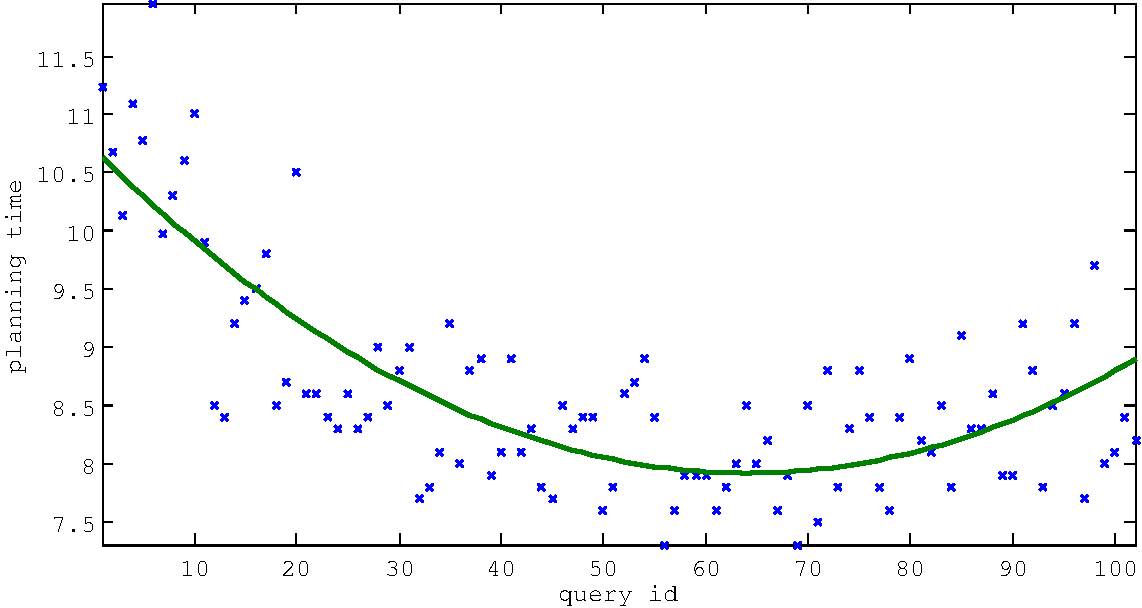
\includegraphics[width=0.8\linewidth]{figs/3/curve1-crop.pdf}
  \caption[Time taken by I-PRM when it runs more than 100 times on the benchmark shown Figure~\ref{fig:3:benchmark}(a). The planning time first decreases and then increases because I-PRM continues updating the dataset in well-learned regions]{\label{fig:3:curve} The time taken by I-PRM when it runs more than 100 times on the benchmark shown in Figure~\ref{fig:3:benchmark}(a). The planning time of a single query first decreases and then increases. The best acceleration acquired is $12.78/7.5 = 70\%$, larger than the $32\%$ in Table~\ref{tab:3:compare}.}
\end{figure}
\begin{figure}[htb]
  \centering
  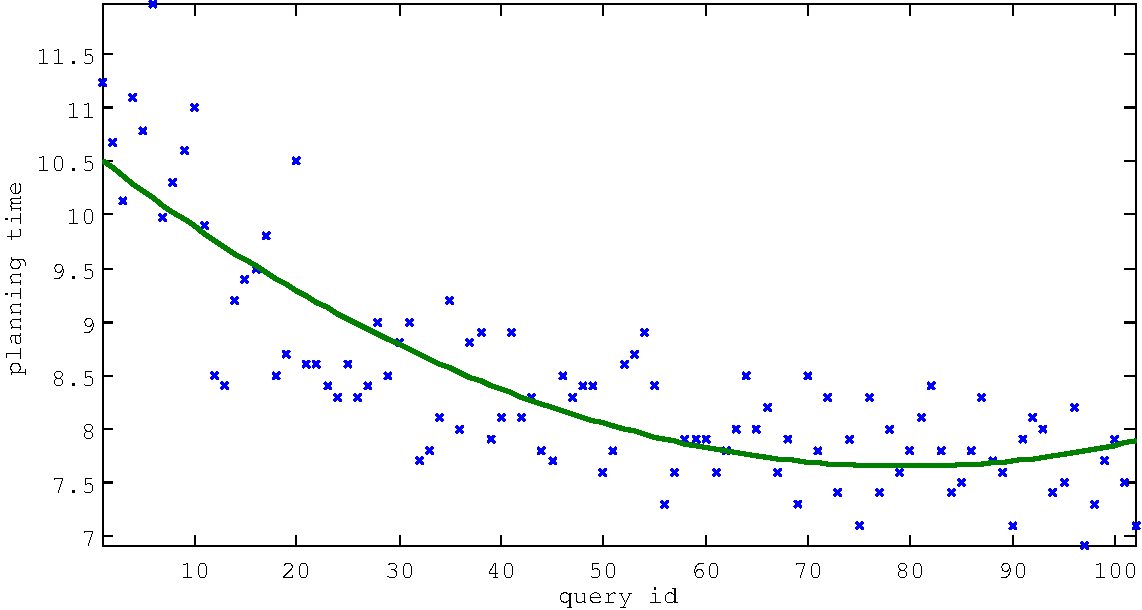
\includegraphics[width=0.8\linewidth]{figs/3/curve2-crop.pdf}
  \caption[Time taken by I-PRM when it runs more than 100 times on the benchmark shown Figure~\ref{fig:3:benchmark}(a). The planning time always decreases because I-PRM stops updating the dataset in well-learned regions]{\label{fig:3:curve2} The time taken by I-PRM when it runs more than 100 times on the benchmark shown in Figure~\ref{fig:3:benchmark}(a). In this experiment, we monitor the average planning time of the most recent $10$ queries and stop adding collision results into the database when average planning time increases. As the database size does not change after about the $60$-th query, the system does not suffer from the re-increase of the planning time. }
\end{figure}



\subsection{Dynamic Environments}
It is possible to extend our method to handle dynamic environments. The underlying obstacle reside in the workspace $W$ ($\mathcal R^2$ or $\mathcal R^3$). We divide the workspace into a set of grids. Then we define two set valued functions,
\begin{align}
\texttt{o\_to\_grid}&: \text{obstacles} \rightarrow \text{collection of grid indices} \notag \\
\texttt{grid\_to\_c}&: \text{grid indices} \rightarrow \text{collection of configurations}. \notag
\end{align}
The function $\texttt{o\_to\_grid}(\text{obstacle})$ returns the indices of the workspace grid cells that overlap with the given obstacle; $\texttt{grid\_to\_c}(\text{grid index})$ returns the set of configuration samples in the database $\mathcal D$ that correspond to the robot colliding with the given grid cell. The two functions can be implemented as two spatial hash tables.

For a moving obstacle, we first find the set of grid cells that overlap with the obstacle's swept volume (between two successive time instances) using function $\texttt{o\_to\_grid}$, and next use $\texttt{grid\_to\_c}$ to get the set of configurations whose collision statuses may change after the movement. Finally, we update the collision statuses for these samples in $\mathcal D$ using exact collision detection. This update operation can be implemented efficiently since our database is implemented as a hash table.


\section{Limitations, Conclusions, and Future Work}

In this chapter, we use instance-based learning to improve the performance of sample-based motion planners. The basic idea is to store the prior collision results as an approximate representation of $\Cobs$ and $\Cfree$, and to replace the expensive exact collision detection query by a relatively cheap probabilistic collision query. We integrate approximate collision routines with various sample-based motion planners and observe $30-100\%$ speedup on rigid and articulated robots.

There are many avenues for future work. First, we need to find methods to adjust LSH parameters adaptively so that the $k$-NN query becomes more efficient for varying dataset sizes. One possible way is to change $L$ (the number of hash tables), because a small $L$ may provide sufficient $k$-NN candidates for a large dataset. Secondly, for samples in regions that are well-explored, we should avoid inserting collision results into the dataset in order to limit the dataset size. Finally, since the prior collision results are stored in hash tables, we can efficiently update the data without high overhead. Therefore, we can extend the instance-based learning framework to improve the performance of planning algorithms in dynamic environments. Moreover, we would like to evaluate the performance in dynamic scenes.



